\title{Rank Techniques and Jump Stratifications}\label{chap6}
\markright{Rank Techniques and Jump Stratifications}

\author{By A. Hirschowitz}
\markboth{A. Hirschowitz}{Rank Techniques and Jump Stratifications}

\date{}
\maketitle

\setcounter{page}{115}

\setcounter{pageoriginal}{158}
IT\pageoriginale IS A fundamental duty and tool for geometers to study
natural stratifications. The theory of special divisors on projective
curves is devoted to such a matter. Much progress has been made in
this field during the last few years (see some references in
\ref{chap6-sec7.2.1}). In the present lecture, I want to emphasize the fact that some
of the tools, which I may call rank techniques and which were
developed mainly for application to questions on special divisors,
have much wider applicability. 

Rank techniques are reviewed in
sections \ref{chap6-sec1}-\ref{chap6-sec4}. In particular the 
rank-Kodaira-Spencer map is introduced in section \ref{chap6-sec3}. It
turns out that many subvarieties in projective spaces are constructed
via rank stratifications (or via similar stratifications). This is
explained in sections \ref{chap6-sec5}, \ref{chap6-sec6}. Jump
stratifications are introduced in section \ref{chap6-sec7} where it is
shown how far the rank techniques are expected to be useful. In
particular, Petri's comorphism is defined, generalizing the Petri's
map of the theory of special divisors.

In section \ref{chap6-sec8}, I give a sample of applications. The
first one should concern special divisors and projective
curves. Instead the reader is invited to see \cite{chap6-Ha}. The
second one computes the number of minimal sections in a general
geometrically ruled surface. The third one is a ``simplification'' in
the proof of the theorem of natural cohomology for rank two vector
bundles over $\mathbb{P}^{3}$ (cf. \cite{chap6-HH2}). And the last one
is an echo from Barth's lecture in the Colloquium: any rank two vector
bundle on $\mathbb{P}^{4}$ with\pageoriginale $c_{1}=1$, $c_{2}=4$ has a two
dimensional family of unstable planes.

From the general definition of jumping loci, the jumping points
emerge. Surprisingly, although considered in several special cases,
the jumping points have not been studied systematically, not even in
the case of curves. Section \ref{chap6-sec9} gives a first account of
this matter.

The results exposed below developed slowly in my mind during my
collaboration with Brun, Hartshorne, Marlin and Narasimhan, for which
I am indebted. This knowledge grew much faster during the two months
after the conference, as I wrote the present paper. I thank the
organizers who gave me the opportunity to think about this in an
accurate way. I also thank them for the kind invitation, and with
them, all those people in the Tata Institute who made my stay so
pleasant.

\section{Rank Stratifications}\label{chap6-sec1}

Many natural stratifications may be viewed as rank stratifications in
the following sense; moreover, the strata of many further natural
stratifications may be viewed as strata of such rank stratifications.

\begin{definition}\label{chap6-defi1.1}
Let $X$ be a quasiprojective smooth connected variety, $E$ and $F$
locally free sheaves on $X$ and $u:E\to F$ a morphism. We define the
rank stratification $X_{u}$ associated with $u$ as follows. First
denote by $p$ the smaller among rank $E$ and rank $F$; then
$X^{i}_{u}$ is defined to be the zero-scheme associated with
$\Lambda^{p-i+1}u$, and the stratification $X_{u}$ is the collection
$(X^{i})_{i\in \mathbb{N}}$.Observe that $X_{u}$ and $X_{u^{*}}$ are
identical\pageoriginale so that we may assume either rank $E=p+\delta$
or as well rank $F=p+\delta$ (with $\delta\geq 0$). We set
$\ring{X}^{i}_{u}:=X^{i}_{u}-X^{i+1}_{u}$. Also we consider the
relative grassmannian variety $G_{E}$ over $X$ of linear subspaces in
the fibers of $E$, and the subscheme $G_{u}$ of subspaces where $u$
vanishes identically. Of course $G_{E}$ (and in general $G_{u}$) have
several connected components corresponding to various dimensions.
\end{definition}

\setcounter{subsection}{1}
\subsection{Program.}\label{chap6-sec1.2}

The study of such a rank stratification splits: from the global study,
we expect answers to the questions: ``What are the non-void strata
$X^{i}_{u}$? What are their degrees, rational equivalence classes,
irreducible components?'' and to similar questions concerning
$G_{u}$. From the local study, we expect answers to be questions:
``What is the maximum rank of $u$? What are the dimensions of the
strata, are they reduced? Are the $X^{i}_{u}$ smooth?'' and to similar
questions concerning $G_{u}$. 

\subsection{Tools.}\label{chap6-sec1.3}

As for the global study : Porteous' formula (Porteous \cite{chap6-P},
Kempf-Laksov \cite{chap6-Kel}) gives the rational equivalence class of
each stratum in terms of Chern classes of $E$ and $F$, provided the
stratum has the expected codimension (namely $i(\delta+i)$ for
$X^{i}_{u}$). This is also a powerful tool to prove existence results
(cf. \cite{chap6-K1L}); and a theorem of
Fulton-Lazarsfeld \cite{chap6-FL} says that in case $X$ is projective,
and $E\spcheck \otimes F$ is ample, then each stratum with positive
expected dimension (i.e. $i(\delta+i)<\dim X$) is connected.

Now locally, rank stratifications are obtained by pulling-back some
universal rank-stratification. Thus the local study splits into the
study of universal rank-stratifications and the study of
base-change. This approach appears in
Arbarello-Cornalba \cite{chap6-AC1}, and both parts are developed in
the next two sections.

\section{Universal Rank
Stratifications {\fontsize{13pt}{15pt}\selectfont\texorpdfstring{\cite{chap6-AC1},\,\cite{chap6-K},\,\cite{chap6-K},\,\cite{chap6-HaT1}}{Cite}}}\label{chap6-sec2}\pageoriginale

\subsection{The Universal Objects.}\label{chap6-sec2.1}

We choose an integer $\delta\geq 0$ and another integer $p>0$, and we
consider the vector space $R_{\delta,p}$ of matrices with $p$ columns
and $p+\delta$ rows, and coefficients in the base field $k$. On
$R_{\delta,p}$ viewed as an affine variety, we have two tautological
morphisms: 
$$
\tau:\mathscr{O}^{p}\to \mathscr{O}^{p+\delta}\quad\text{and}\quad \tau\spcheck
: \mathscr{O}^{p+\delta}\to \mathscr{O}^{p} 
$$
As observed above, the stratifications associated with $\tau$ and
$\tau\spcheck$ are identical. We also denote them with $R_{\delta,p}$
so that $R^{0}_{\delta,p}$ is $R_{\delta,p}$ and the other strata are
the $R_{\delta,p}$'s for $i>0$.

We denote by $G_{\delta,p}$ the connected component \qquad $_{\tau}$
(cf. \ref{chap6-defi1.1}) consisting of subspaces of dimension $i$ and
by $G^{i}_{\delta,p\spcheck}$ the connected component of
$G_{\tau\spcheck}$ consisting of subspaces of dimension $\delta+i$. If
$G$ (resp. $G_{\vee}$)is the grassmannian variety of subspaces of
$k^{p}$ (resp. $k^{p+\delta}$), then $G_{\tau}$
(resp. $G_{\tau\spcheck}$) is a closed subscheme in $G\times
R_{\delta,p}$ (resp.~ $G_{\vee}\times R_{\delta,p}$).

\subsection{Some Properties of \texorpdfstring{$R_{\delta,p}$}{Rdp}.}\label{chap6-sec2.2}

The following properties of $R_{\delta,p}$ are well known :
$\ring{R}^{i}_{\delta,p}$ is smooth of codimension $i(\delta+i)$. For
$i>0$, $R^{i+1}_{\delta,p}$ is the singular locus of
$R^{i}_{\delta,p}$. Each $R^{i}_{\delta,p}$ is reduced, determinantal
and Cohen-Macaulay. On the other hand $G^{i}_{\delta,p}$ and
$G^{i}_{\delta,p\spcheck}$ are smooth and both $G^{i}_{\delta,p}\to
R^{i}_{\delta,p}$ and $G^{1}_{\delta,p\spcheck}\to R^{i}_{\delta,p}$
are (rational) desingularizations of $R^{i}_{\delta,p}$. In case
$\delta=0$, $p=2$, $i=1$, this is the simple example, explained so
long ago by Hironaka, of a threefold with an isolated singularity,
with two minimal desingularizations, the fiber product of which is the
blowing-up of the singular point. Another way to desingularize
$R^{i}_{\delta,p}$ in the general case consists in blowing up
successively\pageoriginale (the strict transform of)
$R^{p}_{\delta,p}$, $R^{p-1}_{\delta,p},\ldots,R^{i+1}_{\delta,p}$. 

Now we review the normal spaces : at a point $u$ in
$\ring{R}^{1}_{\delta,p}$, the normal space is the space of linear
maps $L(\Ker u,\Coker u)$ and the projection of the tangent space to
the normal space is the natural map :
$R_{\delta,p}=L(K^{p},k^{p+\delta})\to L(\Ker u,\Coker u)$. Similarly
at a point $(W,u)$ in $G^{j}_{\delta,p}$, the normal space of
$G^{j}_{\delta,p}$ in $G\times R_{\delta,p}$ is $L(W,k^{p+\delta})$
and the projection from the total tangent space is the natural map
\begin{gather*}
L(W,k^{p}/W)\oplus L(k^{p},k^{p+\delta})\to L(W,k^{p+\delta})\\
(\alpha,\beta)\to \overline{u}\circ \alpha+\beta \circ w,
\end{gather*}
where $w$ is the injection $W\to k^{p}$ and $u$ induces $u$ on
$k^{p}$. The same holds, mutatis mutandis for
$G^{j}_{\delta,p\spcheck}$. 

\subsection{From \texorpdfstring{$R_{\delta,p}$}{Rdp} to
\texorpdfstring{$R_{\delta,p}$}{Rdp}.}\label{chap6-sec2.3}

Let us see that the shape of $R_{\delta,p}$ does not depend too
heavily upon $p$.

\begin{subproposition}\label{chap6-prop2.3.1}
Let $u$ be a point in $\ring{R}^{i}_{\delta,p}$. There exists an open
neighbourhood $U$ of $u$ in $R_{\delta,p}$ and a morphism
$\varphi:U\to L$ ($\Ker u$, $\Coker u$) such that:
\begin{itemize}
\item[\rm(i)] The pull-back by $\varphi$ of the (universal) rank
stratification on 
$$
L(\Ker u, \Coker u)
$$
is the universal rank
stratification $R_{\delta,p}$ restricted to $U$,

\item[\rm(ii)] the derivative $d_{u}\varphi$ of $\varphi$ at $u$ is
the natural projection {\rm (cf. \ref{chap6-sec2.2}).}
\end{itemize}
\end{subproposition}

\begin{proof}
We choose decompositions $k^{p}=\Ker u\oplus A$,
$k^{\delta+p}=\text{Im\,}u\oplus \Coker u$, so that a point $v$ in
$R_{\delta,p}$ reads $v=\left(\begin{smallmatrix} v_{11} & v_{12}\\
v_{21} & v_{22}\end{smallmatrix}\right)$. We\pageoriginale define $U$
to be the open set where $v_{12}$ is an isomorphism. It clearly
contains $u$. And we define $\varphi$ by
$\varphi(v)=v_{21}-v_{22}v^{-1}_{12}v_{11}$. One checks easily (i) and (ii).
\end{proof}

\section{Base Change}\label{chap6-sec3}

The general hope concerning a bundle morphism is that it has maximal
rank (at the generic point) and that the associated
rank-stratification ``looks like'' some universal
rank-stratification. We make precise definitions and then introduce
the rank-Kodaira-Spencer map, in order to give differential criteria
for the above hopes to be fulfilled.

\begin{definition}\label{chap6-defi3.1}
By a stratification indexed by $\mathbb{N}$, I mean a family
$(X^{i})_{i\in \mathbb{N}}$ of (quasi-projective) schemes together
with compatible closed embeddings:
$$
(i<j)X^{j}\hookrightarrow X^{i},
$$
so that the $X^{t}$'s are subschemes of $X^{0}$. The differences
$X^{i}-X^{i+1}$ are locally closed subschemes in $X^{0}$, which we
denote with $\ring{X}^{i}$. Let us say that such a stratification
$(X^{i})_{i\in \mathbb{N}}$ is $R_{\delta}$ -- {\em like at a point}
$x\in \ring{X}^{j}$ if there exists an etale neighborhood $X'$ of
$xX^{0}$ and a smooth morphism $\varphi:X\to R_{\delta,j}$ such that
$(X^{i})_{i\in \mathbb{N}}$ and $R_{\delta,j}$ induce the same
stratification on $X'$. Let us say further that
$(X^{i})_{i\in \mathbb{N}}$ is $R_{\delta}$-like if it is
$R_{\delta}$-like at every point. 
\end{definition}

It follows from \ref{chap6-sec2.3} that for any $\delta$, $p$, the
stratification $R_{\delta,p}$ is $R_{\delta}$-like, and that whenever
a stratification is $R_{\delta}$-like at a point, it is
$R_{\delta}$-like in a neighbourhood.

\setcounter{subsection}{1}
\subsection{The RKS-MAP.}\label{chap6-sec3.2}

Let $u:E\to F$ be a morphism between locally\pageoriginale free
sheaves on the quasi-projective smooth variety $X$. We denote by
$L(E,F)$ the geometric bundle associated with $\Hom(E,F)$, also
usually denoted by $\mathbb{V}(E\otimes F\spcheck)$. Let $\pi$ be the
projection $L(E,F)\to X$. Then over $L(E,F)$, we have a tautological
morphism
$$
\tau_{EF}:\pi^{*}E\to \pi^{*}F
$$
Furthermore, $u$ may be viewed as section of $\pi$ characterized by
$u=u^{*}\tau_{EF}$. 

One checks easily that the rank stratification $(L(E,F)^{i})_{i\geq
0}$ associated with $\tau_{EF}$ is $R_{\delta}$-like where
$\delta=|\rank E-\rank F|$. Also the stratification $X_{u}$ is the
pull-back by (the section) $u$ of the stratification
$(L(E,F)^{i})_{i\geq 0}$. 

Let $O$ be a point in $X$, $E_{O}$ and $F_{O}$ the fibers of $E$ and
$F$ at $O$, and $u_{O}$ the image of $O$ by $u$ in $L(E,F)$. Let $i$
be such that $u_{O}$ is in $L(E,F)^{i}-L(E,F)^{i+1}$. First
$L(E,F)^{i}$ is smooth in $u_{O}$, second it is transversal to the
fibre $\pi^{-1}(O)=L(E_{O},F_{O})$ in $L(E,F)$. Thus the normal space
of $L(E,F)^{i}$ in $L(E,F)$ at $u_{O}$ is canonically identified with
the normal space of $L(E_{O},F_{O})^{t}$ in $L(E_{O},F_{O})$ at
$u_{O}$, which is $L(\Ker u_{O}, \Coker u_{O})$
(cf. \ref{chap6-sec2.2}) so that the differential of $u$ induces a
linear map from the tangent space $T_{0}X$ of $X$ at $O$ into $L(\Ker
u_{0},\Coker u_{0})$. This map we call the rank {\em Kodaira-Spencer
map} (or briefly $RKS$-map) of $u$ at $O$ and we denote it by
$RKS(u,O)$.

\subsection{Criterion for Maximal Rank.}\label{chap6-sec3.3}

Let $A$, $B$, $C$ be vector spaces and $f:A\to L(B,C)$ a linear
map. We shall say that $f$ {\em reaches the maximal rank} if, for a
sufficiently general, $f(a)$ is injective or surjective.

\begin{prop*}
Let $u:E\to F$ be a vector bundle morphism over\pageoriginale a smooth
connected variety $X$. Suppose there exists a point $O$ in $X$ where
$RKS(u,O)$ reaches the maximal rank. Then $u$ has maximal rank (at the
generic point). 
\end{prop*}

\begin{proof}
The statement being local, we may suppose that $E$ and $F$ are
trivial. Also we may suppose that $X$ is a smooth curve. Then $u$
corresponds to an immersion $u:X\to L(k^{p},K^{p+\delta})$. Let us
define $i$ by $u(O)\in \ring{R}^{i}_{\delta,p}$. And let us consider
the map $\varphi$ given by \ref{chap6-sec2.3}. According
to \ref{chap6-sec2.3} ii, the derivative of $\varphi\circ u$ at $O$ is
$RKS(u,O)$ and hence reaches the maximal rank. This means that
$d_{O}(\varphi\circ u)$ takes some values outside of
$R^{1}_{\delta,i}$ which is its own tangent cone. Hence the same is
true of $\varphi\circ u$ itself which, according
to \ref{chap6-sec2.3}.i, implies that $u$ takes some values outside
$R^{1}_{\delta,p}$. 
\end{proof}

\begin{remark*}
We could prove easily, when the field has characteristic zero, that
$RKS(u,x)$ vanishes for $x$ sufficiently general. In particular, if
for any $x$ in $X^{1}_{u}$, $RKS(u,x)$ does not vanish, then $u$ has
maximal rank.
\end{remark*}

\subsection{Criterion for \texorpdfstring{$R_{\delta}$}{Rd}-Likehood}\label{chap6-sec3.4}

\begin{prop*}
Let $X$, $E$, $F$, $\delta$, $u$ be as above. Then $X_{u}$ is
$R_{\delta}$-like at a point $x$ if and only if $RKS(u,x)$ is
surjective. 
\end{prop*}

\begin{proof}
We define $i$ and $\varphi$ as in the previous proof. Then $X_{u}$ is
pulled-back by $\varphi\circ u$ of $R_{\delta,i}$; and the derivative
of $\varphi\circ u$ is $RKS(u,x)$. If the latter is surjective, then
$X_{u}$ is $R_{\delta}$-like at $x$ by definition. On the other hand,
for $(\varphi\circ u)^{*}(O)$ to be smooth of codimension
$i(\delta+i)$ it is necessary that the kernel of $d_{X}(\varphi\circ
u)$ has codimension $i(\delta+i)$, hence that its image has dimension
$i(\delta+i)$. 
\end{proof}


\subsection{Criterion for Smoothness of \texorpdfstring{$G_{u}$}{Gu}
(cf. \texorpdfstring{\cite{chap6-AC1} \ref{chap6-sec3.3}}{Cite}).}\label{chap6-sec3.5}\pageoriginale

\begin{prop*}
Let $X$, $E$, $F$, $\delta$, $u$ and $x$ be as above and let $W$ be a
linear subspace in $\Ker u(x)$ of dimension $i$ if $\rank E\leq \rank
F$, and of dimension $\delta+i$ otherwise. Then $G_{u}$ is smooth of
codimension $i(\delta+i)$ at $W$ in $G_{E}$ (cf.~\ref{chap6-defi1.1})
if and only if $w\circ RKS(u,x)$ is surjective where $w$ is the
restiction map from $L(\Ker u(x),\Coker u(x))$ to $L(W,\Coker u(x))$.
\end{prop*}

\begin{proof}
We suppose, for instance, that $\rank E>\rank F$. Again we consider
(locally) $u$ as a morphism from $X$ to $R_{\delta,p}$. Now $W$
corresponds to a point in $G_{\vee}$ (cf.~\ref{chap6-sec2.1}). We
extend trivially $u$ as a map $\widetilde{u}:G_{\vee}\times X\to
G_{\vee}\times R_{\delta,p}$, so that $G_{\vee}$ is just the pull-back
by $\widetilde{u}$ of $G_{\tau\spcheck}$. Let $\delta+i$ be the
dimension of $W$. Then, as above, the necessary and sufficient
condition for $G_{u}$ to be smooth of codimension $i(\delta+i)$ is
that the derivative $d\widetilde{u}(W,x)$ ranges over the whole normal
space of $G^{i}_{\delta,p\spcheck}$ in $G_{\vee}\times
R_{\delta,p}$. According to \ref{chap6-sec2.2}, this means that the
map
\begin{align*}
&L(W,k^{p+\delta}/W)\oplus T_{x}X\to L(W,k^{p})\\
&
(\alpha,\epsilon)\mapsto \overline{u}\spcheck \circ \alpha+du\spcheck
(x,\epsilon)\circ w 
\end{align*}
is surjective where $w$ is the injection $W\to k^{p+\delta}$ (here we
identify $k^{p}$ and $k^{p+\delta}$ with their duals). Now the image
of $\alpha\mapsto \overline{u}\spcheck \circ\alpha$ is precisely
$L(W,\text{Im\,}u\spcheck)$ so that the condition means that the map
\begin{gather*}
T_{x}X\to L(W,\Coker u\spcheck)\\[3pt]
\epsilon \to \gamma\circ du\spcheck (x,\epsilon)\circ w\quad\text{is
surjective} 
\end{gather*}
where $\gamma$ is the projection $k^{p}\to \Coker u\spcheck$. To
conclude, we just have to observe that $RKS(u,x)(\epsilon)$ is the
composition 
$$
\Ker u\spcheck \to k^{p+\delta}\xrightarrow{du\spcheck
(x,\epsilon)}k^{p}\to \Coker u\spcheck. 
$$\pageoriginale
\end{proof}

\section{Stable Properties \texorpdfstring{\cite{chap6-BH2}}{Cite}}\label{chap6-sec4}

In \cite{chap6-BH2}, Brun and I emphasized stable properties of
stratifications. In this section, after recalling the definitions, we
review $R_{\delta}$-likehood from this point of view of stability.

\subsection{Definitions.}\label{chap6-sec4.1}

Although everybody understands what is meant by a property being
satisfied by stratifications indexed by $\mathbb{N}$, let us give a
careful definition: let us say that it is a subset of the set of
isomorphism classes of stratifications indexed by $\mathbb{N}$. Now we
say that a property $P$ (satisfied by $(X^{t})_{i\in \mathbb{N}}$ as
soon as there exists an \'etale covering $(X_{\alpha})_{\alpha\in A}$
of $X^{\circ}$ such that $P$ is enjoyed by each induced stratification
$(X^{i}\alpha)_{i\in \mathbb{N}}$. Finally we say that the property
$P$ is {\em stable} if, whenever it is satisfied by a stratification
$(T^{i})_{i\in \mathbb{N}}$ with $T^{0}$ smooth, it also holds: 
\begin{itemize}
\item[(a)] for any submersion $R\to T^{0}$, by the induced
stratification $(R^{i})_{i\in \mathbb{N}}$,

\item[(b)] for any submersion $T^{0}\to R$, with $R$ connected, by the
induced stratification on the general fiber $T^{0}(r)$.
\end{itemize}

\setcounter{examples}{1}
\begin{examples}
Here are the most usual examples:
\begin{itemize}
\item[(a)] $X^{i}$ is $s$-codimensional in $X^{0}$.

\item[(b)] $\ring{X}^{i}$ is smooth.

\item[(c)] $X^{i}$ is locally complete intersection.

\item[(d)] $X^{i}$ is determinantal.

\item[(e)] $X^{i+1}$ is the singular locus of $X^{i}$.

\item[(f)] locally, in the \'etale topology, $X^{i}$ is trivial along
$X^{i+1}$. 

\item[(g)] $X^{p+1}$\pageoriginale is empty, and $X^{i}$ may be
desingularized by blowing-up successively (the strict transforms of)
$X^{p}$, $X^{p-1},\ldots,X^{i+1}$ (cf.~\ref{chap6-sec2.2}).
\end{itemize}
\end{examples}

\setcounter{subsection}{2}
\subsection{Stability of \texorpdfstring{$R_{\delta}$}{Rd} - Likehood.}\label{chap6-sec4.3}

\begin{prop*}
$R_{\delta}$-likehood is a stable property.
\end{prop*}

\begin{proof}
The property is clearly stable under submersions. Hence we may
consider a submersion $s:X\to Y$ where $X$ is endowed with the
stratification induced by another submersion $f:X\to
L(k^{j},k^{\delta+j})$. By Bertini's theorem, the general fiber
$Z=s^{-1}(y)$ intersects transversally the strata $\ring{X}^{i}$. Let
$x$ be a point in $Z\cap \ring{X}^{i}$. We know that around $x$, the
stratification on $X$ is induced by a submersion $f':X\to
L(k^{i},k^{\delta+i})$. Since $Z$ is transversal to the special fiber
$X^{i}$ of $f'$, the restriction of $f'$ to $Z$ is again a submersion,
which proves that the stratification induced on $Z$ is
$R_{\delta}$-like at $x$.
\end{proof}

\setcounter{subremark}{3}
\begin{subremark}\label{chap6-rem4.4}
Another point of view is as follows. Call any local stable property
satisfied by every $R_{\delta,p}$ a stable property satisfied by
$R_{\delta}$. Then one proves easily that a stratification indexed by
$\mathbb{N}$ is $R_{\delta}$-like if and only if it satisfies all the
stable properties of $R_{\delta}$. Of course $R_{\delta}$ is not a
stratification itself. However, as pointed out by M.F. Atiyah, it may
be thought of as the stratification by the corank of the open set of
Fredholm operators with index $\delta$ in the Hilbert space (of course
only in the complex case.) Stratification on infinite dimensional
manifolds is a main tool in Atiyah-Bott \cite{chap6-AB} (see
also \cite{chap6-Ki}). 
\end{subremark}

\section{Other Stratifications}\label{chap6-sec5}

There are several other standard ways to construct stratifications
with corresponding universal stratifications and KS-maps. We briefly
review two of them.

\subsection{Symmetric Rank-Stratifications
(\texorpdfstring{\cite{chap6-C}, \cite{chap6-B4}}{Cite})}\label{chap6-sec5.1}\pageoriginale

Instead of general morphisms $u:E\to F$, we consider symmetric
morphisms $\mu:E\to E\spcheck$. The universal stratifications are
induced by $R_{0,n}$ on the vector subspaces of symmetric maps in
$L(k^{n},k^{n})$. The range of the $KS$-map is the vector space
$L_{s}(\Ker u_{O}\Coker u_{O})$ of symmetric linear maps from $\Ker
u_{O}$ to $\Coker u_{O}$ (since $u_{O}$ is symmetric, $\Ker u_{O}$ and
$\Coker u_{O}$ are dual to each other). 

\subsection{\texorpdfstring{$\Sigma$}{S}-Stratificatons
(\texorpdfstring{\cite{chap6-Mu}, \cite{chap6-Su}}{Cite}).}\label{chap6-sec5.2} 

Let $Y\to X$ be a locally (in the \'etale topology) trivial bundle
over $X$ with typical fiber $\mathbb{P}^{1}$. Let $E$ be a rank-two
vector bundle over $Y$. The splitting type of the restriction
$E|_{Y(x)}$ of $E$ to the fiber defines a (scheme) stratification of
$X$. The corresponding universal stratifications live on
semi-universal deformations of rank two vector bundles over
$\mathbb{P}^{1}$. These split into two families $\Sigma^{0}$ and
$\Sigma^{1}$ according to the parity of the degrees. As in the rank
case, one can define $\Sigma^{0}$-like and $\Sigma^{1}$-like
stratifications. In the present case, the $KS$-map is the classical
one with values in $H^{1}(Y(O), \End E(O))$.

According to Gruson-Peskine (\cite[p.1]{chap6-GP3}), the corresponding
universal stratifications may also be seen as rank stratificatons on
vector spaces of so-called per-symmetric matrices. 

\subsection{\texorpdfstring{$S$}{S}-Likehood.}\label{chap6-sec5.3}

In each of the case we have encountered so far, instead of a single
universal stratification, we have seen a sequence of universal
stratifications (which we could glue over a Hilbert manifold,
see \ref{chap6-rem4.4}). So the following definition seems relevant. 

\begin{defi*}
Let $S$ be a set of stratifications, each indexed by $\mathbb{N}$ and
let $(X^{i})_{i\in \mathbb{N}}$ be a further stratification. We say
$(X^{i})_{i\in \mathbb{N}}$ is $S$-like\pageoriginale in case it
enjoyes any local stable property enjoyed by any member of $S$.
\end{defi*}

For this definition to fit with that of $R_{\delta}$-likehood, we have
to consider $R_{\delta}$ as the set $\{R_{\delta,p}\}_{p>0}$. 

\section{Constructing Subvarieties}\label{chap6-sec6}

After having worked some time on vector bundles (or any other topic)
one asks himself why. The answer, though not immediate, arises, in
general, from connections with other fields whose interest is
presumably more clear. I am satisfied with the connection between
vector bundles and subvarieties say of projective spaces. First vector
bundles are a tool in the study of subvarieties. Second, vector
bundles provide new natural varieties through their moduli. Finally,
many subvarieties are constructed starting from vector bundles. The
original idea was to consider zero-sets of sections of vector
bundles. It turns out that several generalizations of this idea deal
with rank stratifications. That is what is explained in the present
section. 

\subsection{Zero-Sets.}\label{chap6-sec6.1}

It is a standard tool, called the Serre-Horrocks construction and
reactived by Barth - van de Ven \cite{chap6-BV1}, \cite{chap6-BV2} in the
seventies. Given a rank two vector bundle $E$ and a section $s$, we
get an exact sequence:
$$
0\to \mathscr{O}_{f}\xrightarrow{s}E\to I_{Y}(c_{1})\to 0.
$$
Provided $s$ just vanishes in codimension two, $I_{Y}$ is the ideal
sheaf of $s^{-1}(0)$ and $c_{1}$ is the determinant of $E$. This is,
on the one hand, a starting point for studying vector bundles and
their
moduli \cite{chap6-H2}, \cite{chap6-L1}, \cite{chap6-HS}, \cite{chap6-Bru}, \cite{chap6-E}
through subvarieties and their Hilbert scheme and, on the other hand,
this is a tentative technique\pageoriginale to find out
subvarieties \cite{chap6-HoM}. Here is a picture of corresponding
properties for vector bundles and from subvarieties point of view
(over projective space):
\begin{center}
\renewcommand{\arraystretch}{1.3}
\begin{tabular}{p{3.7cm}|c|p{3.7cm}}
\hline
Subvarieties side & connection & vector bundles side\\
\hline
$Y$ smooth & $(\exists)$ $\Longleftarrow$ & $E$ globally
generated\\
$Y$ connected & $\Longleftrightarrow$ & $h^{1}(E(-c_{1}))=0$\\
postulation\newline $h^{\circ}(I_{Y}(s))$ & $\leftrightsquigarrow$ &
cohomology\newline $h^{\circ}(E(s-c_{1}))$\\
liaison & $\Longleftarrow$ & twist, cf.~ \cite{chap6-Ra1}, \cite{chap6-Ra2}\\
cohomology of the\newline normal bundle & $\leftsquigarrow$ & cohomology of
$E(s)$,\newline $E\otimes E(s)$, cf.~\cite{chap6-BE2}\\
compactification:\newline Hilbert scheme & \raisebox{-.7cm}{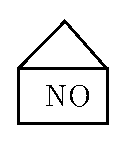
\includegraphics[scale=.6]{1.eps}} &
compactification:\newline Maruyama's moduli \\[-.3cm]
&&\\
\hline 
\end{tabular}
\end{center}

\subsection{First Generalization.}\label{chap6-sec6.2}

Suppose we have a linear algebraic group $G$ acting (linearly) on
$k^{N}$ and a stratification $S=(S^{i})_{i\in I}$ of
$\mathbb{A}^{N}_{k}$ (i.e. $S^{\circ}=\mathbb{A}^{N}_{k}$), which is
invariant under the action of $G$. Suppose we have a rank $N$ vector
bundle on $X$ with structure group $G$. Then the total space
$\mathbb{V}(E\spcheck)$ inherits a stratification $(E^{i})_{i\in I}$,
locally induced by $(S^{i})_{i\in I}$ through
trivializations. Furthermore, if $\sigma$ is a section of $E$ over
$X$, viewed as section of $\mathbb{V}(E\spcheck)\to X$ it induces a
stratification $X_{\sigma}$ defined by $X^{i}_{\sigma}=\sigma\ast
E^{i}$. Now this is used through the following general nonsense: 

\begin{prop*}[(cf. \cite{chap6-K1}, \cite{chap6-Vo})]
In\pageoriginale case $E$ is globally generated (i.e.~
$$
H^{0}(E)\otimes \mathscr{O}\to E
$$ 
is surjective) and $\sigma$ is
general enough, then $X_{\sigma}$ is $S$-like {\rm
(cf. \ref{chap6-sec5.3})}. In particular, if $S$ is a universal rank
stratification $R_{\delta,p}$ then $X_{\sigma}$ is $R_{\delta}$-like. 
\end{prop*}

\begin{proof}
Let $e:H^{0}(E)\times X\to \mathbb{V}(E\spcheck)$ be the evaluation
map. Since $E$ is globally generated, $e$ is a submersion. For
$\sigma$ in $H^{0}(E)$, $X_{\sigma}$ is the stratification induced by
$e^{*}(E^{i})_{i\in I}$ on $\{\sigma\}\times X$. The projection
$H^{0}(E)\times X\to H^{0}(E)$ is again a submersion. Thus the
statement follows from the definition of stability.
\end{proof}

\noindent
{\bf Program.}~
In order to invoke this proposition, one has to
\begin{itemize}
\item[(a)] choose the group $G$, the representation and the
stratification (supposed to be well known).

\item[(b)] find a globally generated vector bundle with structure
group $G$ acting through the chosen representation. One way, for
instance, if $G=GL(n,k)$, is to start with a globally generated rank
$n$ vector bundle and consider the rank $N$ vector bundle associated
with the representation. If the representation is suitably
``positive'', this vector bundle will be globally generated
again. Also remember (\cite[p.~99]{chap6-Mum}) that for $E$ to be
globally generated, a sufficient condition (on $\mathbb{P}^{n}$) is 
$$
0=H^{1}(E(-1))=H^{2}(E(-2))=\ldots=H^{n}(E(-n)).
$$

\item[(c)] study global properties of the obtained strata. Here
methods of (\ref{chap6-sec1.2}), or analogous methods should be helpful.
\end{itemize}


\subsection{Examples}\label{chap6-sec6.3}

\subsubsection{}\label{chap6-sec6.3.1}
We first see how zero sections fit into this frame. Here $G=GL(n,k)$,
the representation is the identity, and the stratification is:
$$
S^{0}=\mathbb{A}^{n},\quad S^{1}=0\in \mathbb{A}^{n}.
$$\pageoriginale

\subsubsection{}\label{chap6-sec6.3.2}

Here $G=GL(V)$ acts diagonally on $V^{r}$, and $N=nr$. The
stratification is by the rank (observe $V^{r}=L(k^{r},V)$). In case we
have $r\leq n$ and $d<2(n-r+2)$ where $d$ is the dimension of $X$,
this leads to smooth subvarieties of codimension $n-r+1$
(\cite{chap6-Vo}, \cite{chap6-Ra2}, \cite{chap6-Sch}, \cite{chap6-HeS}).

\subsubsection{}\label{chap6-sec6.3.3}

More generally, $G=GL(V)\times GL(W)$ acts on $L(V,W)$ and the
universal rank stratification is invariant. We just come back to rank
stratifications as introduced in \ref{chap6-defi1.1} to
which \ref{chap6-sec6.2} applies whenever $\scrHom(E,F)$ is generated
by global sections. Examples over $\mathbb{P}^{3}$ with $E$ and $F$
sums of line bundles arise in \cite{chap6-E11}. Let us observe that
the main theorem in \cite{chap6-HH2}, giving many vector bundles
globally generated over $\mathbb{P}^{3}$ leads to much more curves
than suggested in (\cite[p.~365]{chap6-HH2}). More generally, this technique
would yield many smooth subvarieties of dimension $d$ in
$\mathbb{P}^{n}$, for roughly $2d\leq n$, if we could prove that there
are many globally generated vector bundles over $\mathbb{P}^{n}$ at
least in higher rank.

\subsubsection{}\label{chap6-sec6.3.4}

Here $G=GL(V)$ acts on $S^{2}V,N=\dfrac{n(n+1)}{2}$. The
stratification is again by the rank (cf.~\ref{chap6-sec5.1}). This
leads to hypersurfaces with a 3-codimensional signular locus of double
points, provided the base dimension is at most 5
(cf.~\cite{chap6-C}, \cite{chap6-B4}). Furthermore there is an
extension of Porteous' formula available for this
case \cite{chap6-JLP}, \cite{chap6-Tu}, \cite{chap6-HaT1}, \cite{chap6-HaT2}.

\subsection{Second Generalization}\label{chap6-sec6.4}

Previous considerations extend in some sense to sheaves with tame
singularities. In the rank two case over a 3-fold, suitable sheaves
are reflexive sheaves of which the number of singular points is
precisely the third Chern class. Starting from such a globally
generated sheaf, the\pageoriginale method of \ref{chap6-sec6.3.1} leads
to nonsingular curves \cite{chap6-HH0}, while the method
of \ref{chap6-sec6.3.4} leads to surfaces with
nodes \cite{chap6-HM}. 

\section{Jump Stratifications (cf.~ \texorpdfstring{\cite[\S\
1]{chap6-BH2}}{Cite})}\label{chap6-sec7}

Many stratifications occurring in the theory of vector bundles or in
the theory of subvarieties of projective spaces are what we define
below as jump stratifications. In the present section, we explain how
far rank stratification techiniques help in their study. In
particular, we generalize Petri's map which, in good cases, describes
the first order local behaviour of the jump stratification for
semi-universal families.

\begin{definition}\label{chap6-defi7.1}
Let $\pi:X\to S$ be a projective morphism and $(E_{\alpha})_{\alpha\in
A}$ be a finite set of $S$-flat coherent sheaves over $X$. According
to the semi-continuity theorem, the dimensions
$h^{i}(E_{\alpha,X(s)})$ define upper semi-continuous integer-valued
functions on $S$. All together, these functions define on $S$ the jump
stratification associated with $(E_{\alpha})_{\alpha\in A}$. For the
moment, the jump stratification is set-theoretic. An additional scheme
structure may be defined, at least in the cases we are interested
in. Also, observe that the jump stratification is not indexed for the
moment; or, it is indexed by the huge set of integer valued functions
on $I\times A$ where $I=\{0,\ldots,n\}$ and $n$ is the (maximal)
dimension of the fibers of $\pi$. Indeed, for such a function $g$, we
may set
$$
S^{g}=\left\{s\in S\mid \forall i\quad \forall \alpha, h^{i}(E_{\alpha\
X(s)})\geq g(i,\alpha)\right\}.
$$
\end{definition}

\setcounter{subsection}{1}
\subsection{Examples}\label{chap6-sec7.2}

\subsubsection{Special Divisors}\label{chap6-sec7.2.1}

This is the fundamental example: $S$ is the Jacobian variety of
isomorphism classes of line bundles of degree $d$ over a smooth
projective curve $C$ and $X$ is $C\times S$. Finally,\pageoriginale
$E$ is some Poincar\'e bundle over $X$
(cf.~e.g. \cite{chap6-GH2}, \cite{chap6-G} \cite{chap6-FL}, \cite{chap6-EH1},
\cite{chap6-EH2}, \cite{chap6-T} and for an
introduction \cite{chap6-Ha}).

\subsubsection{Postulation}\label{chap6-sec7.2.2}

$S$ is a subvariety of the Hilbert scheme of $\mathbb{P}^{n}$, $X$ is
$S\times \mathbb{P}^{n}$; we denote by $U$ the universal subscheme and
by $I_{U}$ its ideal sheaf. The considered sheaves are $I_{U}(l)$,
$\mathscr{O}_{U}(l)$, $l$ running in a big subset of $\mathbb{Z}$
(outside of which nothing happens)
(cf. e.g. \cite{chap6-E11}, \cite{chap6-GP1}, \cite{chap6-GP2}, \cite{chap6-GLP}, \cite{chap6-H3}, \cite{chap6-HH1}, \cite{chap6-Hi}, \cite{chap6-BE1}, \cite{chap6-BE3}, \cite{chap6-BE4}, \cite{chap6-BH4}).

\subsubsection{Jump Loci}\label{chap6-sec7.2.3}

Let $Y$ be a projective variety and $(\mathscr{F}_{\alpha})_{\alpha\in
A}$ a finite set of vector bundles over $Y$ (for instance a set of
twists $E(1)$ of a single bundle $E$). Let $S$ be a subvariety in the
Hilbert scheme of $Y$, with universal subscheme $U$ and corresponding
ideal sheaf $I_{U}$. We consider the jump stratification associated
with the sheaves $\mathscr{F}_{\alpha}\boxtimes I_{U}$,
$\mathscr{F}_{\alpha}\boxtimes \mathscr{O}_{U}$ (cf. \cite{chap6-BH1},
\cite{chap6-BH2}, \cite{chap6-BH3}, \cite{chap6-Ch}, \cite{chap6-BHM}). This
stratification is a fundamental tool in the classification of vector
bundles over projective
spaces \cite{chap6-Schw}, \cite{chap6-VdV}, \cite{chap6-BV1}, \cite{chap6-BV2}, \cite{chap6-B2}, \cite{chap6-B3}, \cite{chap6-Hu1}.

\subsubsection{Line Subbundles Over Curves}\label{chap6-sec7.2.4}

Let $S$, $C$, $X$, $E$ be as in \ref{chap6-sec7.2.1} and let $F$ be a
rank two vector bundle over $C$. Then the jump stratification
associated with $E\spcheck \boxtimes F$ distinguishes line subbundles
of $F$
(cf. \cite{chap6-N}, \cite{chap6-Ma1}, \cite{chap6-St}, \cite{chap6-Gu},
\cite{chap6-LN}, \cite{chap6-Ray}). One of the obtained strata is the
starting point for the classification of (semi-) stable rank two
vector bundles over $C$
(cf.~ \cite{chap6-NR1}, \cite{chap6-NR2}, \cite{chap6-NR3}). 

\subsubsection{Normal Bundles}\label{chap6-sec7.2.5}

Let $S$ be a subvariety of the Hilbert Scheme of smooth space curves
and $X\subset S\times \mathbb{P}^{3}$ be the tautological curve. The
normal bundle $N$ is a rank two vector bundle over $X$. Among the
twisted bundle $N(l):=N\boxtimes \mathscr{O}_{\mathbb{P}^{3}(\ell)}$,
$N(-1)$ stands out as the only one with zero Euler-Poincare
characteristic.\pageoriginale Hence it will be the most sensitive to
jump phenomena. So we are interested in the jump stratification
associated with $N(-2)$
(cf.~ \cite{chap6-GS}, \cite{chap6-S1}, \cite{chap6-EV1}, \cite{chap6-EV2},
\cite{chap6-EL}, \cite{chap6-HuS}, \cite{chap6-El}, \cite{chap6-BE2}, \cite{chap6-E1H},
\cite{chap6-Hu2}). One has also studied the restricted tangent bundle
and other restricted standard
bundles \cite{chap6-V}, \cite{chap6-Br}, \cite{chap6-Ki}.

\subsubsection{Stratification of Quot-Schemes}\label{chap6-sec7.2.6}

Let $(Y,Y,(1))$ be a projective variety, $\mathscr{F}$ a coherent
sheaf over $Y$ and $H$ a (Hilbert) polynomial. This defines a
Grot-scheme $S$ of quotients of $\mathscr{F}$ with Hilbert polynomial
$H$. Over $X=S\times Y$ we have the universal quotient, the universal
subsheaf and their twists. This situation
generalizes \ref{chap6-sec7.2.2}. 

\subsection{Generalization}\label{chap6-sec7.3}

We want to consider some among the above situations with
parameters. For instance, in \ref{chap6-sec7.2.1}, we want to consider
$C$ as a point in the moduli of curves. The hope here is to understand
in a better way the original stratification as the trace of a
(well-understood) stratification on something bigger. Some trouble
arises because in general there is no Poincare bundle over moduli
see \cite{chap6-NR1}, \cite{chap6-R}, \cite{chap6-LP1}, \cite{chap6-HN}, \cite{chap6-Me}, \cite{chap6-MR}. Fortunately,
in order to define jump stratifications, we only need sheaves up to
line bundles over $S$. So we could define a pseudo-$S$-sheaf over $X$
to be a section over $S$ of the sheaf in the etale topology associated
with the presheaf $P$ for which $P(T)$ is the set of isomorphism
classes of sheaves over $X_{T}$, modulo $\Pic T$. The obstruction for
a pseudo-$S$-sheaf over $X$ to come from a sheaf is in
$H^{2}_{\text{\'et}}(S,\mathscr{O}_{S}\ast)$. Now, on the one hand,
jump-stratifications are clearly defined for pseudo $S$-sheaves and on
the other, there exists a (unique) Poincar\'e (pseudo-$S$-sheaf on
$S\times Y$ whenever $S$ is a moduli of stable sheaves on $Y$. So the
new picture is $E_{\alpha}\to X\to S\to M$ where $E_{\alpha}$ is a
pseudo-$S$-sheaf and where $M$ stands to remind us that we are
interested not only in the stratification over $S$ but also in its
restriction to the fibers\pageoriginale of $S\to M$. Observe that we
get a natural stratification on $M$ by flattening the jump
stratification on $S$.

\subsection{Examples}\label{chap6-sec7.4}

\subsubsection{}\label{chap6-sec7.4.1}
Example \ref{chap6-sec7.2.1} extends by letting $C$ move in the moduli
of curves (rigidified in such a way that the relative Jacobian
exists). The corresponding stratification on the moduli $M$ selects
the hyperelliptic locus, the trigonal locus, and so on.

\subsubsection{}\label{chap6-sec7.4.2}
Example \ref{chap6-sec7.2.3} extends by letting the sheaves
$\mathscr{F}_{\alpha}$ move in their moduli. In this way, we get a
stratification (by jumping loci) on moduli say of stable vector
bundles (see an example of result concerning this stratification
in \cite[Prop. 5.2]{chap6-LP2}).

\subsubsection{}\label{chap6-sec7.4.3}
Examples \ref{chap6-sec7.2.4} extends by letting the vector bundle $F$
move in some moduli. The corresponding stratification of the moduli is
finer than by the degree of stability (cf. \cite{chap6-LN}).

\subsubsection{}\label{chap6-sec7.4.4}
Notations are those of \ref{chap6-sec7.2.5}. Let $J\to S$ be a
relative Jacobian associated with $X\to S$ and $P$ a Poincar\'e
(pseudo-$J$-) bundle over $\fprod{J}{X}{S}$. We consider the
(pseudo-$J$-) sheaf $\scrHom(P,N)$ on $\fprod{J}{X}{S}$. The
corresponding stratification on $M:=S$ is finer than by the degree of
stability of $N$ (cf.~ \cite{chap6-S2}, \cite{chap6-Ne}).

\subsubsection{}\label{chap6-sec7.4.5}
$S$ is a moduli of stable vector bundles over a projective variety
$Y$, $X$ is $S\times Y$, and $E$ is a Poincar\'e (pseudo-$J$-) sheaf
on $S\times Y$. This is another generalization of \ref{chap6-sec7.2.1}
(cf.~ \cite{chap6-B3}, \cite{chap6-H2}, \cite{chap6-H4}, \cite{chap6-Bru}, \cite{chap6-L1}, \cite{chap6-HH2}, \cite{chap6-BH3}). 

\subsection{Programme}\label{chap6-sec7.5}

In order to describe a jump stratification, the first task
consists\pageoriginale in discovering the generic value of the
$h^{i}$'s. This is the corresponding maximal rank problem. Here the
general hope is that the generic value should be minimal among values
suitable for the Riemann-Roch formula (cf. for
instance \cite{chap6-BH3}). The next step is to find a simpler way of
indexing. The hope here is that very few among the $h^{i}$'s should be
relevant, preferably only two, related by Riemann-Roch. Observe here
that among a family of twisted sheaves $E(l)$, the most sensitive to
jump phenomena should be the ones for which the Hilbert polynomial
$\chi(E(l))$ assumes its minimal absolute value. In any case, one
should discover all the possible values of the $h^{i}$'s. The final
hope is to identify strata as strata of some rank stratification for
which the techiniques reviewed above could help, the goal being, of
course, to find degrees, rational equivalence classes, irreducible (or
connected) components of the strata, and to describe the local shape.

\subsection{Global Tools}\label{chap6-sec7.6}

For the rest of the present section, we suppose that we are concerned
with a single torsion-free sheaf $E$ such that the restrictions
$E|_{X(S)}$-are torsion-free too and that we know that, for any $s\in
S$, and any $i\geq 2$, $h^{i}(E|_{X(s)})$ vanishes. Then
$h^{0}(E|_{X(s)})-h^{1}(E|_{X(s)})$ is a constant $\chi$. Moreover the
jump stratification is a rank stratification. Indeed, we can embed $E$
in a vector bundle $F$ with no higher direct images
(i.e. $R^{i}\pi\ast F=0$, $i>0$) in such a way that the restricted
morphisms $E|_{X(s)}\to F|_{X(s)}$ are injections too. Then the
cokernel $G$ of $E\to F$ is flat and has no higher direct images as
well because, for $i>1$, $R^{i}\pi_{\ast}E$ vanishes. By the
Riemann-Roch formula, $h^{0}(F|_{X(s)})$ and $h^{0}(G|_{X(s)})$ are
locally constant. Thus, by the base change theorem, $\pi_{\ast}F$ and
$\pi_{\ast}G$ are locally free and the jump stratification fits with
the rank stratification associated with
$u:\pi_{\ast}F\to \pi_{\ast}G$. Incidentally, our stratification
acquires a scheme structure (which according to the theory of
Fitting\pageoriginale ideals does not depend upon the choice of $E\to
F$). So the global tools of \ref{chap6-sec1.3} apply. More precisely,
in case $X$ and $S$ are smooth, the rational equivalence classes of
the strata $S^{i}$, supposed to have the right dimension $i(|\chi|+i)$
where $\chi^{1}$ is the Euler-characteristic of $E(s)$, are, modulo
torsion given by an expression of the form $\Delta_{i}$
$(\log(\pi_{\ast}(\text{ch~ }E.\ \text{td~} X/S)))$ where $td$ is the
Todd class, ch is the Chern character, $\log$ is a universal
polynomial map from $A^{*}(S)\otimes \mathbb{Q}$ into itself and
$\Delta$; another one, depending on the index of the stratum
(cf. \cite{chap6-GP3}, \cite{chap6-BS}, \cite{chap6-BH3}).

\subsection{Petri's Morphisms}\label{chap6-sec7.7}

For the study of the local behavior, we still require the assumptions
of \ref{chap6-sec7.6} and suppose further that $E$ is locally free and
that $\pi:X\to S$ is trivial (say for simplicity). Then at any point
$s\in S$, we have:
\begin{itemize}
\item[--] the map $RKS(u,s):T_{s}S\to L(H^{0}(E(s)),H^{1}(E(s)))$

\item[--] the deformation $KS$ map:
$$
DKS(E,s):T_{s}S\to H^{1}(X(s),\End E(s))
$$
\end{itemize}

\noindent
{\em Petri's comorphism:}
$$
PC(E(s)):H^{1}(X(s),\End E(s))\to L(H^{0}(E(s)),H^{1}E(s))):
$$
this is the natural map associated with $E(s)\otimes \End E(s)\to
E(s)$. I call it comorphism because, in the theory of special
divisors, Petri's map is the dual of the present map. As one would
expect (up to sign!), we have:

\begin{prop*}
$RKS(u,s)=-PC(E(s))\circ DKS(E,s)$.
\end{prop*}

\begin{proof}
Here we set $X=Y\times S$ and we may suppose that the bundle $F$
introduced in \ref{chap6-sec7.6} is of the form $\pr_{1}\ast F'$. We
may suppose $S=\Spec (k[\epsilon]/\epsilon^{2})$. So we have exact
sequences: 
\begin{gather*}
0\to E\to \pr^{*}_{1}F'\xrightarrow{q}G\to 0\\
0\to H^{0}(E(O)\to H^{0}(F')\to
H^{0}(G(O))\xrightarrow{\alpha}H^{1}(E(O))\to 0.
\end{gather*}\pageoriginale 
Over the generic point $y$ of $Y$, we can choose a splitting:
$$
F'(y)=E(O)(y)\oplus G(O)(y).
$$


We know that the tangent space to $\Quot F$ corresponding to $G(O)$ is
$\Hom(E(O),G(O))$ and that the image of the canonical tangent vector
of $S$ in this tangent space is a map $\varphi:E(O)\to G(O)$ such that
over $\{y\}\times S$, $E$ is the graph, in $(S\times E(O)(y))\times
G(O)(y)\subset S\times F')$, of $\epsilon \varphi$. Now let $\gamma$
be a section of $E(O)$, and let $\sigma$ be the corresponding constant
section of $\pi_{\ast}F$. We want to compute $q(\sigma)$. Over the
generic point $y$, $\sigma(y)+\epsilon\varphi(\sigma(y))$ is a section
of $E(y)$, so that $q(\sigma(y)+\epsilon\varphi(\sigma(y)))=0$. This
implies that $q(\sigma)=-\epsilon\varphi(\sigma)$. Now $DKS(E,s)$ is
known to be the image of $\varphi$ under the natural map
$$
\beta : \Hom(E(O),G(O))\to \Ext^{1}(E(O),E(O))
$$
and we conclude because for any section $\delta$ of $E(O)$, the
following diagram is commutative:
\[
\xymatrix{
\Hom(E(O),G(O))\ar[d]^{\circ\gamma}\ar[r]^-{\beta}
& \Ext^{1}(E(O),E(O))\ar[d]^{\gamma^{\ast}}\\
\Hom(\mathscr{O},G(O))=H^{0}(G(O))\ar[r]^-{\alpha} &
H^{1}(E(O))=\Ext^{1}(\mathscr{O},E(O)). 
}
\]
\end{proof}

\begin{remarks*}
\begin{itemize}
\item[(a)] Hence the surjectivity of the $RKS$-map follows if we know
the surjectivity of the $DKS$-map {\em and} of Petri's comorphism.

\item[(b)] Similar considerations hold in case, instead of $h^{0}$,
$h^{1}$, only the\pageoriginale highest group $h^{n}$, $h^{n-1}$ are
not identically zero. Also, by duality, one can pass from one case to
the other. 
\end{itemize}
\end{remarks*}

\section{Applications}\label{chap6-sec8}

One of the main applications of the techniques reviewed above is to
the study of space curves. In the first version of the present text, I
devoted a section to it. Then my attention was drawn
to \cite{chap6-Ha} where this study is performed much more
completely. That is why there is no section 8.1 below.

\setcounter{subsection}{1}
\subsection{Ruled Surfaces}\label{chap6-sec8.2}

Let $C$ be a curve of genus $g$ and $E$ be a stable rank two vector
bundle over $C$, of degree $d$. Let $J$ denote the Jacobian of $C$ and
$P$ be a Poincar\'e bundle over $J\times C\to J$ of relative degree
$d'$. Consider over $J\times C$ the bundle
$\Hom(P,p^{\ast}_{2}E)$. The associated jump stratification on $J$
selects classes of line bundles which inject (as sheaves) in $E$. Now
a theorem of Nagata (\cite{chap6-N}, see
also \cite{chap6-St} \cite{chap6-Gu} \cite{chap6-LN} \cite{chap6-L2})
says that whenever $d'\leq \dfrac{d-g+1}{2}$, such line bundles
exist. This result could be reproved in the vein
of \cite{chap6-K1L}. Instead, we give the following sample.

\begin{theorem*}
If $C$ and $E$ are general enough, and $d-g$ is odd, then $E$ as
exactly $2g$ subbundles of degree $\dfrac{d-g+1}{2}$.
\end{theorem*}

\begin{proof}
We may suppose $d=g-1$ and set $\alpha=\left[\dfrac{g}{2}\right]$,
$\alpha'=g-\alpha$ so that $\alpha\leq \alpha'\leq \alpha+1$. We may
suppose that Petri's condition holds for $C$. This implies that for
any line bundle $L$ over $C$ of degree $\alpha$ or $\alpha'$, we have
$h^{0}(C,L)\leq 1$. Now we choose two line bundles $L_{\alpha}$ and
$L_{\alpha'}$ of degree $\alpha$ and $\alpha'$ and set
$E_{0}=L_{\alpha}\oplus L_{\alpha'}$. We consider the semi universal
deformation of $E_{0}$: this is a vector bundle $E$ over $S\times C$
where $S$ is a smooth variety with base\pageoriginale point $O$, such
that the fiber $E(O)$ is $E_{O}$ and the tangent space $T_{O}S$ is
identified with $H^{1}(C,\End E_{0})$ (cf. \cite{chap6-KS} or for a
sketch of the algebraic proof \cite{chap6-Bi}). Now, we denote by $J$
the Jacobian of $C$, and by $P$ a Poincar\'e bundle over $J\times C$
of relative degree $0$, and we consider the bundle $\Hom(P,E)$ over
$J\times S\times C$ as a family of bundles over $C$ parametrized by
$J\times S$. I claim that the associated jump stratification is
$R_{g-1}$-like along $J\times \{O\}$. Indeed, its $R.K.S$ map at a
point $L\times \{O\}$, restricted to the subspace $\{O\}\times T_{o}S$
of the tangent space $T_{L}J\times T_{o}S$ is the natural map
$$
H^{1}(\End E_{O})\to L(H^{o}(L\spcheck \otimes E_{O}),
H^{1}(L\spcheck \otimes E_{O})). 
$$

In order it prove that it is surjective, we prove that its four parts
are surjective namely:
\begin{gather*}
u_{1}:H^{1}(\End L_{\alpha})\to L(H^{0}(L\spcheck \otimes L^{q}),
H^{1}(L\spcheck \otimes L_{\alpha}))\\[3pt]
u_{2}:H^{1}(\End L_{\alpha'})\to L(H^{0}(L\spcheck \otimes
L_{\alpha'}), H^{1}(L\spcheck \otimes L_{\alpha'}))
\end{gather*}
are surjective by Petri's assumption on $C$ and 
\begin{align*}
& u_{3}:H^{1}(\Hom(L_{\alpha},L_{\alpha'}))\to
L(H^{0}(L\spcheck \otimes L_{\alpha}), H^{1}(L\spcheck \otimes
L_{\alpha'}))\\[3pt]
& u_{4}:H^{1}(\Hom(L_{\alpha'},L_{\alpha}))\to
L(H^{0}(L\spcheck \otimes L_{\alpha'}), H^{1}(L\spcheck \otimes L_{\alpha}))
\end{align*}
are transposed in
\begin{gather*}
u^{*}_{3}:H^{0}(L\spcheck \otimes L_{\alpha})\otimes
H^{0}(\Omega\otimes L\spcheck_{\alpha'}\otimes L)\to
H^{0}(\Omega\otimes L_{\alpha}\otimes L\spcheck_{\alpha'})\\[3pt]
u^{*}_{4}:H^{0}(L\spcheck\otimes L_{\alpha'})\otimes
H^{0}(\Omega\otimes L\spcheck_{\alpha}\otimes L)\to
H^{0}(\Omega\otimes L_{\alpha'}\otimes L\spcheck_{\alpha})
\end{gather*}
which are injective because $h^{0}(L\spcheck \otimes L_{\alpha})\leq
1$, $h^{0}(L\spcheck\otimes L_{\alpha'})\leq 1$. Hence
by \ref{chap6-sec4.3}, for $s$ general in $S$, the jump stratification
associated with\break 
$\Hom(P,E(s))$ is $R_{g-1}$-like. This means that
$E(s)$ has a finite number $n$ of subbundles of degree $0$ and this
number\pageoriginale is given by Porteous' formula
(cf.~\ref{chap6-sec7.3}). Now we prove $n=2^{g}$. It is proved
in \cite{chap6-K1L}, although not explicitly stated, that if $P'$ is a
Poincar\'e bundle over $C\times J$ of relative degree $d>2g-2$ on the
fibers of $C\times J\to C$, and of relative first Chern class $0$ on
the fibers of $C\times J\to C$, then the Chern class of
$\mathfrak{p}_{\ast}P'$ is
$\exp(-\theta)=1-\theta+\dfrac{\theta^{2}}{2}+\cdots$ modulo numerical
equivalence, where $\theta$ is the polarization class. In order to
compute the Chern class of $p_{2!}(E_{O}\otimes {P'}\spcheck)$, we
choose a very negative line bundle $L_{\beta}$ so that the line bundle
$L'_{\beta}:=(\det E_{O})\otimes L\spcheck_{\beta}$ is very
positive. One checks easily that $E_{O}$ is a generalization of
$E_{1}:=L_{\beta}\oplus L_{\beta'}$, so that we compute Chern class of
$p_{2!}(E_{1}\otimes {P'}\spcheck)$, which is
$$
C(p_{2\ast}(L'_{\beta}\otimes
{P'}\spcheck))/C\spcheck(p_{2*}(\Omega\otimes L_{\beta}\otimes P'))
$$
and by the quoted result, the inverse Chern class is $\exp (2\theta)$
whose top component $2^{g}$ is the number we look for.
\end{proof}

\begin{remark*}
This was known to Segre (cf. \cite{chap6-WG1}). For a more general
formulation of the problem solved above, see \cite{chap6-WG2}. 
\end{remark*}

\subsection{Cohomology of Instanton Bundles}\label{chap6-sec8.3} 

The maximal rank problem for the moduli of rank two stable vector
bundles over $\mathbb{P}^{3}$ is solved in \cite{chap6-HH2}, at least
in one irreducible component of each moduli $M(c_{1},c_{2})$. The
proof consists in looking at a non-locally free specialization of some
simple bundles in order to reduce the problem to a suitable general
position statement. We show how this reduction can be achieved
using \ref{chap6-sec3.3} instead of specialization (this was known to
Hartshorne long ago):

\begin{prop*}
Let $a=2$ (resp. $a=3$). Suppose that there exists a disjoint union
$Y\subset \mathbb{P}^{3}$ of $r$ lines (resp. conics) and a morphism
$\beta:\mathscr{O}(-a)\to \mathscr{O}_{Y}$ such that for all
$n\in \mathbb{Z}$, taking $\alpha=(\beta,\rho)$, the induced maps 
\begin{gather*}
H^{0}(\alpha(n)):H^{0}(\mathbb{P}^{3},\mathscr{O}(n-a)\oplus \mathscr{O}(n))\to
H^{0}(Y,\mathscr{O}_{Y}(n))\quad\text{and}\\[3pt]
H^{0}(\rho(n)):H^{0}(\mathbb{P}^{3},\mathscr{O}(n))\to
H^{0}(Y,\mathscr{O}_{Y}(n)) 
\end{gather*}\pageoriginale
are of maximal rank. Then there exists a rank two vector bundle $E$
over $\mathbb{P}^{3}$ with natural cohomology and $c_{1}(E)=0$ (resp
$-1$), $c_{2}(E)=r-1$ (resp. $2r-2$). 
\end{prop*}

\begin{proof}
We choose a vector bundle $E_{O}$ sitting in an extension
$$
0\to \mathscr{O}(1-a)\to E_{O}\to I_{Y}(1)\to 0.
$$
Such an $E_{O}$ exists and it corresponds to a smooth point in the
moduli (cf. \cite{chap6-H2}). Hence, according to \ref{chap6-sec3.3}
and \ref{chap6-sec7.7}, it is enough to prove that $PC(E_{O}(l-1))$
reaches the maximal rank, for each $l$. We see that
$H^{1}(E_{O}(l-1))=H^{1}(I_{Y}(l-1))$. If this group vanishes there is
nothing to prove; so, we may suppose that $H^{0}(I_{Y}(l-1))$
vanishes. Then we see that
$H^{0}(E_{O}(l-1)=H^{0}(\mathscr{O}(l-a))$. We also see that

$\Ext^{1}(E_{O},E_{O})\to \Ext^{1}(E_{O},I_{Y}(1))$ is surjective as
well as 

$\Ext^{1}(E_{O},I_{Y}(1))\to \Ext^{1}(\mathscr{O}(1-a),I_{Y}(1))$ and

$\Hom(\mathscr{O}(1-a),\mathscr{O}_{Y}(1))\to \Ext^{1}(\mathscr{O}(1-a),I_{Y}(1))$. We
choose $\beta$ in $\Ext^{1}(E_{O},E_{O})$ having the same image in
$\Ext^{1}(\mathscr{O}(1-a),I_{Y}(1))$ as $\beta$, and we check that
the assumption on $\beta$ implies that
$PC(E_{O}(l-1))(\overline{\beta})$ has maximal rank.
\end{proof}

\begin{remark*}
The general position statement in \cite{chap6-HH2} is weaker since
only the first series of maps is required to have maximal
rank. However, the second series of maps is known to have
maximal\pageoriginale rank for a general union of
lines \cite{chap6-HH1}, and should not be too difficult to handle for
a general union of $r\geq 3$. Moreover, this approach fits in a better
way with \cite{chap6-H3} p. 109.
\end{remark*}

\subsection{Unstable Planes}\label{chap6-sec8.4}

Let $E$ be a vector bundle over $\mathbb{P}^{n}$, $n\geq 3$ with rank
$E=2$, $-1\leq c_{1}(E)\leq 0$ and let $\chi=2+c_{1}-c_{2}$. Then $E$
is expected to have at least a $(|\chi|+1)$-codimensional family of
unstable planes (i.e. planes $H$ for which $H^{0}(E_{H})\neq 0$)
provided a certain polynomial in $c_{2}$ (with coefficients depending
on $n$, $c_{1}$, $\chi$) does not vanish. This polynomial can be
computed in any case, given time. We give an example corresponding to
Barth's lecture.

\begin{prop*}
Any rank two vector bundle over $\mathbb{P}^{4}$ with $c_{1}=-1$,
$c_{2}=4$ has at least a two-dimensional family of unstable planes. 
\end{prop*}

\begin{proof}
In case there exists a two-dimensional family of planes $H$ with
$H^{2}(E_{H})\neq 0$, we are done because, by Serre-duality, such
planes are unstable. So we suppose that the family of such planes is
at most one-dimensional. Let $G'$ be the complement of this family in
the grassmannian variety of planes in $\mathbb{P}^{4}$. Over $G'$, the
family of restrictions of $E$ satisfies the conditions
of \ref{chap6-sec7.6}. Hence it is enough to prove that the expected
rational equivalence class is not zero in $G'$. Although
straightforward, the computation seems quite tedious. Fortunately, we
can avoid it thanks to \cite{chap6-BHM}. Indeed, they prove that the
family of unstable planes of the Horrocks-Mumford bundle $F$ is
non-empty and two-dimensional. In order to conclude, it is sufficient
to prove that for any plane $H$, $H^{2}(F_{H})$ vanishes. And this
follows \cite{chap6-Hu2}, because $F(3)$ is globally generated outside
25\pageoriginale lines, and has a section with exactly 6 zeroes on
each of these lines, so that, for any $H$, $F_{H}(3)$ has a section
vanishing in codimension two. From the eact sequence
$$
0\to \mathscr{O}_{H}\to F_{H}(3)\to I_{Y}(5)\to 0
$$
we deduce $H^{0}(F_{H}(-2))=0$ which, by Serre-duality, implies the
desired result. 
\end{proof}

\begin{remark*}
It was announced during the Colloquium that someone (in USSR) has
constructed a rank two vector bundle on $^{4}$ with $c_{1}=-1$,
$c_{2}=4$, which is not isomorphic to a Horrocks-Mumford bundle. 
\end{remark*}

\section{Jumping Points}\label{chap6-sec9}

Let $Y$ be a projective non-singular variety, and $E$ a vector bundle
over $Y$ (or $(E(l))_{l\in A}$ a set of twists of $E$). We may
consider $Y$ as a subvariety in its own Hilbert scheme either in the
trivial way (simple points) or as a variety of non-reduced points (big
points, see \ref{chap6-sec9.1}). According to \ref{chap6-sec7.2.3}, we
get corresponding jump stratifications on $Y$ itself. Jumping points
in $Y$ are points in the non-dense strata. While jumping lines
appeared as a fundamental tool from the very beginning of the theory
of vector bundles over projective spaces
(see \cite{chap6-Schw}, \cite{chap6-VdV}, \cite{chap6-BV1}, \cite{chap6-BV2}),
jumping points were considered in a much more discrete way
(see \ref{chap6-sec9.2}). The general hope here around is to describe
(stable) vector  bundles (and consequently their moduli) in terms of
some of their jumping loci together with possible additional data
living there. The prototype is Barth's
result \cite[\S\ 2.3.4]{chap6-B3} (See
also \cite[\S\ 7.2, 7.3]{chap6-Hu1}). From this point of view, the
current knowledge about $M_{\mathbb{P}^{3}}(-1,2)$ \cite{chap6-HS} and
$M_{\mathbb{P}^{3}}(0,2)$ \cite{chap6-H3} is quite satisfactory. In
case of more involved moduli, one has to study\pageoriginale each
stratum separately (see e.g. \cite{chap6-BM}). In this section, after
some generalities, we look at some examples of loci of jumping simple
points (\ref{chap6-sec9.2}), then we solve the maximal rank problem
for big points jumping with respect to rank two stable vector bundles
on $\mathbb{P}^{2}$ with even first Chern class (\ref{chap6-sec9.3}).

\subsection{Generalities}\label{chap6-sec9.1}

Let $Y$, $E$ be as above, and let $d$ be the dimension of $Y$, and $r$
be the rank of $E$. Choose an integer $s\geq 0$ and define an
$s$-big-point in $Y$ to be the subscheme associated with the
$(s+1)$-th power of a maximal ideal sheaf. So, for $s=0$, an
$s$-big-point is just a (simple) point. For each $s$, if we set
$N(s)=\binom{s+d}{s}$, we have an embedding $Y\to \Hilb^{N(s)}Y$,
corresponding to $s$-big-points. The corresponding universal
sub-scheme $U_{s}$ in $Y\times Y$ is the $s$-th infinitesimal
neighbourhood of the diagonal. We see that the only sensible groups
are $H^{0}(E\boxtimes I_{U_{s}}(y))$ and $H^{1}(E\boxtimes
I_{U_{s}}(y))$ and that the jump stratification is the rank
stratification associated with
$$
\ev_{s}:H^{0}(E)\otimes \mathscr{O}_{Y}\to J^{s}E
$$
where $J^{s}E$ is the jet-bundle:
$J^{s}E=\pr_{-1\ast}(E\otimes\mathscr{O}U_{s})$; and $\ev_{s}$ is the
corresponding evaluation. 

So we are interested in the Chern polynomial $c_{t}(J^{s}E)$. From the
exact sequences. 
$$
0\to S^{s}\Omega \otimes E\to J^{s}E\to J^{s-1}E\to 0,
$$
we get $c_{t}(J^{s}E)=\prod\limits^{s}_{l=0}c_{t}(S^{-1}\Omega \otimes
E)$, where $S^{l}\Omega$ is the $l$-th symmetric power of the
cotangent bundle. Also we observe that sensitive $s$ will achieve
small values of $|h^{\circ}(E)-rN(s)|$. 

\subsection{Simple Points}\label{chap6-sec9.2}

The jump locus of simple points first occurred in the study of
unstable rank two vector bundles over $\mathbb{P}^{2}$\pageoriginale
(Grauert-Mulich \cite{chap6-GM}). For stable bundles, it appeared in
the study of special moduli over $\mathbb{P}^{3}$, rather than over
$\mathbb{P}^{2}$. 

\begin{subexample}\label{chap6-exam9.2.1}
$M_{\mathbb{P}^{3}}(0,2)$, cf. Hartshorne \cite{chap6-H3}, see
also \cite{chap6-HN}. Rank two stable bundles over $\mathbb{P}^{3}$
with $c_{1}=2$, $c_{2}=3$ have two sections whose dependency locus is
a smooth quadric $Q$. The bundle and its other jumping loci (lines,
planes) are described in terms of a certain pencil over this jumping
locus $Q$. 
\end{subexample}

\begin{subexample}\label{chap6-exam9.2.2}
$M_{\mathbb{P}^{3}}(-1,2)$, cf. Hartshorne-Sols \cite{chap6-HS}, see
also \cite{chap6-M}, \cite{chap6-MW}. Rank two stable bundles over
$\mathbb{P}^{3}$ with $c_{1}=1$, $c_{2}=2$ have (up to scalars) only
one non-zero section whose zero scheme is a double line. This jumping
locus plays the central role in the classification. For the similar
study of $M_{\mathbb{P}^{3}}(-1,4)$, see \cite{chap6-BM}. 
\end{subexample}

\begin{subexample}\label{chap6-exam9.2.3}
$M_{\mathbb{P}^{2}}(1,2)$. A rank two stable bundle $E$ over
$\mathbb{P}^{2}$ with $c_{1}=1$, $c_{2}=2$ has two sections whose
dependency locus is a line $L$ (the unique jumping line). The image of
$H^{0}(E)$ in $E|_{L}$ is a line bundle of degree two over $L$ so that
$H^{0}(E)$ defines a pencil of degree two. The two double points in
this pencil characterize $E$. The second kind of jumping lines are the
lines through one among these two points (see \cite[p. 236]{chap6-LP1}
and \cite[p. 256]{chap6-Hu1}).
\end{subexample}

\begin{subexample}\label{chap6-exam9.2.4}
$M_{\mathbb{P}^{2}}(0,4)$. A general rank two stable bundle $E$ over
$\mathbb{P}^{2}$ with $c_{1}=2$, $c_{2}=5$ has two sections whose
dependency locus is a smooth conic, where they define a pencil of
degree 5. Jumping lines are lines cutting the conic in two points of a
divisor in the pencil. 
\end{subexample}

\begin{subexample}\label{chap6-exam9.2.5}
$M_{\mathbb{P}^{2}}(0,5)$. A general rank two stable bundle $E$ over
$\mathbb{P}^{2}$ with $c_{1}=2$, $c_{2}=6$ has (up to scalars) only
one non-zero section, vanishing at six points
(see \cite[p. 84]{chap6-B3}). 
\end{subexample}

\begin{remark*}
The\pageoriginale jumping loci considered
in \ref{chap6-exam9.2.4}, \ref{chap6-exam9.2.5} lead to a nice
description of an open dense subset in the moduli which generalizes to
cases where the Euler-Poincar\'e characteristic is two or one. 
\end{remark*}

\subsection{Jumping Big-Points}\label{chap6-sec9.3}

\subsubsection{Line Bundles over Curves}\label{chap6-sec9.3.1}

Let $L$ be a general line bundle of degree $d\geq g$ over a curve $C$
of genus $g$. We have a morphism from $C$ into its Jacobian of degree
$g-1$ through $x\mapsto [L(-(d+1-g)x)]$. The intersection with the
$\theta$-divisor gives $g(d+1-g)^{2}$ points. This is the jump locus
for $(d+1-g)$-big points. 

\subsubsection{Rank Two Vector Bundles Over \texorpdfstring{$\mathbb{P}^{2}$}{P2}, With
Even \texorpdfstring{$c_{1}$}{c1}}\label{chap6-sec9.3.2}

What we saw in \ref{chap6-exam9.2.4}, \ref{chap6-exam9.2.5} generalizes
to the case of big points as soon as the Euler-Poincar\'e
characteristic is of the form $s^{2}+s-1$, $s^{2}+s$ or
$s^{2}+s+1$. To see that the corresponding jumping loci are actually
non-trivial, we have to solve a maximal rank problem, namely

\begin{theorem*}
Let $c_{1}$, $c_{2}$ be integers with $c_{1}$ even and
$c^{2}-4c_{2}\leq -8$. Then, for the general rank two stable vector
bundle $E$ over $\mathbb{P}^{2}$ with Chern classes $c_{1}$, $c_{2}$,
the evaluations
$$
\ev_{s}:H^{0}(E)\otimes \mathscr{O}\to J^{s}E
$$
have maximal rank.
\end{theorem*}

\begin{proof}
First, remember \cite{chap6-Schw}, \cite{chap6-Ma2} that the required
condition on $c_{2}$ is necessary and sufficient for the moduli
$M_{\mathbb{P}^{2}}(c_{1},c_{2})$\pageoriginale of rank two stable
vector bundles with these Chern classes to be non-empty, and that this
moduli is irreducible. Next remember that an open dense subset in the
moduli consists of classes of bundles with ``natural'' cohomology
(cf. eg. \cite{chap6-Bru}). Now, observe that if $\ev_{s}$ is
injective, so is $\ev_{t}$ for any $t>s$. Also, observe that the
property for $\ev^{-}_{s}$ to have maximal rank is open in flat
families of torsion free sheaves $\mathscr{F}_{t}$ with constant
$h^{0}(\mathscr{F}_{t})$. So it is sufficient to prove that for any
$s$, there exists a bundle $E$ in $M_{\mathbb{P}^{2}}(c_{1},c_{2})$
with natural cohomology and $\ev_{s}$ of maximal rank. In fact, it is
sufficient to produce a torsion-free sheaf $\mathscr{F}$ satisfying:
\begin{itemize}
\item[(i)] $\ev_{s}:H^{0}(\mathscr{F})\otimes \mathscr{O}\to
J^{s}\mathscr{F}$ has maximal rank

\item[(ii)] $H^{1}(\mathscr{F})=0$ (or $H^{0}(\mathscr{F})=0$).

\item[(iii)] $\mathscr{F}$ deforms to a rank two stable bundle with
Chern classes $c_{1}$, $c_{2}$. 
\end{itemize}
The Euler-Poincar\'e characteristic for our bundles is
$$
\chi =2^{\frac{1}{2}}c_{1}(c_{1}+3)+2-c_{2}.
$$

So we may suppose $c_{1}>0$, $c_{2}<\frac{1}{2}c_{1}(c_{1}+3)+2$,
otherwise, for the general $E$, $H^{0}(E)$ vanishes.

First, we let $c_{1}=2t$, and set $c_{2}=t^{2}+2d+\epsilon$ with
$0\leq \epsilon\leq 1$. We know $d\geq 0$. We choose
$\mathscr{F}=I_{X}(t)\oplus I_{Y}(t)$ where $X$ is a general set of
$d$ points in $\mathbb{P}^{2}$ and $Y$ a general set of $d+\epsilon$
points in $\mathbb{P}^{2}$. So we have
$0\leq \chi(I_{X}(t))-\chi(I_{Y}(t))\leq 1$ and
$\chi(I_{X}(t))+\chi(I_{Y}(t))=\chi$. So for $X$ and $Y$ general
enough, $H^{1}(\mathscr{F})$ vanishes. Now (i) and (ii) follow from
the lemmas:
\end{proof}

\begin{lemma}\label{chap6-lem1}
For a sufficiently general subset $Z$ in $\Hilb^{d}\mathbb{P}^{2}$,
$$
\ev_{s}:H^{0}(I_{Z}(t))\otimes \mathscr{O}-J^{s}(I_{Z}(t))
$$ 
has maximal rank. 
\end{lemma}

\begin{lemma}\label{chap6-lem2}
Let\pageoriginale $t$, $d_{1}$, $d_{2}$ be integers satisfying
$$
\dfrac{(t-2)(t-1)}{2}<d_{1}\leq d_{2}\leq \dfrac{t(t+1)}{2}
$$
and for $i=1$, $2$ let $Y_{i}$ be in $\Hilb^{d} \
{}^{i}\mathbb{P}^{2}$. Then $I_{Y_{1}}\oplus I_{Y_{2}}$ deforms to a
stable vector bundle. 
\end{lemma}

\noindent
{\bf Proof of Lemma \ref{chap6-lem1}.}
It is enough to prove that the general union $T$ of one $s$-big point
and $d$ points has maximal rank (i.e. the restrictions
$$
H^{0}(\mathbb{P}^{2},\mathscr{O}(l))\to H^{0}(\mathbb{P}^{2},\mathscr{O}_{T}(l))
$$
have maximal rank). Adding or deleting points, it is enough to treat
the case where $d=0$ (evident) or 
$$
\dfrac{(l+1)(l+2)}{2}=\dfrac{s(s+1)}{2}+d.
$$
Observe that $s+d\geq l+1$. Thus we may choose $l+1-s$ points on a
line meeting the $s$-big point and we proceed by induction in the
usual way (cf. \cite{chap6-HH1}, \cite{chap6-Hi}). 

\smallskip
\noindent
{\bf Proof of Lemma \ref{chap6-lem2}.}
We may suppose $Y_{1}$ and $Y_{2}$ smooth and general so that for any
point $p$ in $Y_{i}$,
$H^{0}(I_{Y_{i}-\{\mathfrak{p}\}}(t-3))=0$. Thus, there exist exact
sequences (cf. \cite{chap6-GH1}, \cite{chap6-Bru}):
$$
0\to \mathscr{O}\to E_{i}\to I_{Y_{i}}(t)\to 0
$$
where $E_{1}$, $E_{2}$ are locally free, Furthermore, we have
\begin{gather*}
H^{1}(E_{i}(-1))=H^{1}(I_{Y_{i}}(t-1))=0\\[3pt]
\text{and}\quad H^{2}(E_{i}(-2))=H^{2}(I_{Y_{i}}(t-2))=0. 
\end{gather*}
Hence,\pageoriginale by Castelnuovo's criterion
(\cite[p. 99]{chap6-Mum}), $E_{i}$ is generated by global
sections. Now we have an exact sequence
$$
0\to \mathscr{O}\oplus \mathscr{O}\xrightarrow{u_{0}}E_{1}\oplus
E_{2}\to I_{Y_{1}}(t)\oplus I_{Y_{2}}(t)\to 0.
$$
Moving $u_{0}$ in the vector space
$L(\mathscr{O}\oplus \mathscr{O},E_{1}\oplus E_{2})$ we get a
deformation of $I_{Y_{1}}(t)\oplus I_{Y_{2}}(t)$ which is flat,
because the Hilbert polynomial is constant (cf. \cite{chap6-H1}
III. 9.9 and its proof). Now by \ref{chap6-sec6.2}, for general $u$,
$\Coker u$ is locally free. So $I_{Y_{1}}\oplus I_{Y_{2}}$ deforms to
a vector bundle as well and this vector bundle, by semicontinuity has
no non-zero section hence is stable. 

\begin{remarks*}
A similar statement and proof should hold in case $c_{1}$ is odd and
also over $\mathbb{P}^{3}$ at least for the so-called general
instanton bundle. 
\end{remarks*}

\begin{thebibliography}{}
\bibitem{chap6-AC1} E. Arbarello - M. Cornalba : Su una congettura di
Petri. {\em Comment. Math. Helvetici} 56 (1981), 1-38. 

\bibitem{chap6-AC2} E. Arbarello -- M. Cornalba : A few remarks about variety of irreducible plane curves of given degree and genus, {\em Ann. Scient. Ec. Norm. Sup.,} 16 (1983) 467-488.

\bibitem{chap6-AB} M.F. Atiyah - R. Bott : The Yang-Mills equations over Riemann surfaces, {\em Phil. Trans. R. Soc. Lond.} A 308, (1982) 523-615.

\bibitem{chap6-BE1} E. Ballico\pageoriginale - Ph. Ellia : Generic curves of small genus in $\mathbb{P}^{3}$ are of maximal rank, {\em Math. Ann.,} 264 (1983) 211-225.

\bibitem{chap6-BE2} E. Ballico - Ph. Ellia : Some more examples of curves in $\mathbb{P}^{3}$ with stable normal bundle, {\rm J. Reine Angew. Math.,} 350 (1984), 87-93.

\bibitem{chap6-BE3} E. Ballico - Ph. Ellia : Sur la postulation des courbes de $\mathbb{P}^{n}$ et de leurs projections, {\em C.R.A.S.} Paris, 299 (1984), 237-240.

\bibitem{chap6-BE4} E. Ballico - Ph. Ellia : The Maximal rank conjecture for non-special curves in $P^{3}$, {\em Invent. Math.,} 79 (1985) 541-555.

\bibitem{chap6-BM} C. Banica - N. Manolache : Rank 2 stable vector bundles on $\mathbb{P}^{3}(C)$ with Chern classes $c_{1}=1$, $c_{2}=4$, Preprint, Bucarest (1983). 

\bibitem{chap6-B1} W. Barth : Submanifolds of low codimension in projective space, {\em Proceedings of the International Congress of Mathematicians,} Vancouver, 1974, 409-413.

\bibitem{chap6-B2} W. Barth : Some properties of stable rank-2 vector bundles on $\mathbb{P}_{n}$, {\em Math. Ann.,} 226, 125-150 (1977).

\bibitem{chap6-B3} W. Barth : Moduli of vector Bundles on the projective plane. {\em Invent. Math.,} 42, 63-91 (1977).

\bibitem{chap6-B4} W. Barth : Counting singularities of quadratic forms on vector bundles, in {\em Vector Bundles and Differential Equations,} Prog. in Math., 7 Birkhauser, Boston 1980, 1-19.

\bibitem{chap6-BHM} W. Barth\pageoriginale - K. Hulek - R. Moore : Shioda's modular surface $S(5)$ and the Horrocks-Mumford bundle. These Proceedings, 1984.  

\bibitem{chap6-BV1} W. Barth - A. Van de Ven : A decomposability criterion for algebraic 2-bundles in projective spaces, {\em Invent. Math.,} 25 (1974), 91-106. 

\bibitem{chap6-BV2} W. Barth - A. Van de Van : On the geometry in codimension 2 of Grassmann manifolds, {\em Springer L. N. in Maths.} 412, Springer-Verlag (1974), 1-35.

\bibitem{chap6-BS} J. Bertin - I. Sols : Quelques formules \'enum\'eratives concernant les fibres vectoriels sur $\mathbb{P}^{r}$, {\em C.R.A.S.,} Paris, 294 (1982), 197-201.

\bibitem{chap6-Bi} J. Bingener : Appendix in \cite{chap6-BH2}.

\bibitem{chap6-Br} A. Bruguieres : Le sch\'ema des morphismes d'une courbe elliptique dans une grassmannienne, These 3e cycle, Paris VII (1984).

\bibitem{chap6-Bru} J. Brun : Les fibr\'es de rang dues sur $\mathbb{P}_{2}$ et leurs sections, {\em Bull. Soc. Math. France}, 108 (1980) 457-473.

\bibitem{chap6-BH1} J. Brun - A. Hirschowitz : Droites de seut des fibr\'es stable de rang \'elev\'e sur $\mathbb{P}_{2}$, {\em Math. Zeit,} 181 (1982), 171-178. 

\bibitem{chap6-BH2} Vari\'et\'es des droites sauteuses du fibr\'e instanton g\'en\'eral, {\em Compos. Math.,} 53 (1984), 325-336. 

\bibitem{chap6-BH3} J. Brun\pageoriginale - A. Hirschowitz : Restrictions planes du fibre instanton general I, II, In preparation.

\bibitem{chap6-BH4} J. Brun - A. Hirschowitz : Sur la stratification par la postulation du schema de Hilbert de $\mathbb{P}^{2}$, Preprint, Nice (1984).

\bibitem{chap6-C} F. Catanese : Babbage's conjecture, contact of surfaces, symmetrical determinant varieties and applications, {\em Invent. Math.,} 63 (1981), 433-465.

\bibitem{chap6-Ch} M.C. Chang : A bound on the order of jumping lines, {\em Math. Ann.,} 262 (1983), 511-516.

\bibitem{chap6-E} L. Ein : Some stable vector bundles on $\mathbb{P}^{4}$ and $\mathbb{P}^{5}$, {\em J. Reine Angew. Math.,} 337 (1982), 142-153.

\bibitem{chap6-EH1} D. Eisenbud - J. Harris : A simpler proof of the Gieseker-Petri theorem on special divisors, {\em Invent. Math.,} 74 (1983), 269-280.

\bibitem{chap6-EH2} D. Eisenbud - J. Harris : Divisors on general curves and cuspidal rational curves, {\em Invent. Math.,} 74 (1983), 371-418.

\bibitem{chap6-EV1} D. Eisenbud - A. Van de Ven : On the normal bundle of smooth rational space curves, {\em Math. Ann.,} 256 (1981), 453-463.

\bibitem{chap6-EV2} D. Eisenbud - A. Van de Ven : The irreducibility of the space of rational space curves with given degree and normal bundle, {\em Invent. Math.,} 67 (1982), 89-100.

\bibitem{chap6-El} Ph. Ellia : Examples de courbes de $\mathbb{P}^{3}$ a fibre normal semi-stable, stable, {\em Math. Ann.,} 264 (1983) 389-396.

\bibitem{chap6-E11} G. Ellingsrud :\pageoriginale Sur le sch\'ema de Hilbert des vari\'eti\'es de codimension 2 dans $\mathbb{P}^{e}$ \'a c\^one de Cohen-Macaulay, {\em Ann. Sci. Ecole Norm. Sup. Paris,} 8 (1975), 423-432.

\bibitem{chap6-E1H} G. Ellingsrud - A. Hirschowitz : Sur le fibr\'e normal des courbes gauches, {\em C.R.A.S.,} Paris, 299 (1984), 245-248.

\bibitem{chap6-EL} G. Ellingsrud - D. Laksov : The normal bundle of elliptic space curves of degree five, in  {\em 18th Scand. Congress of Math. Proc.} 1980, Prog. in Math., {\em 11} Birkh\"auser, Boston, 1981, 258-287.

\bibitem{chap6-FL} W. Fulton - R. Lazarsfeld : On the connectedness of degeneracy locus and special divisors, {\em Acta Math.,} 146 (1981), 271-283.

\bibitem{chap6-GS} F. Ghione - G. Sachiero : Normal bundles of rational curves, {\em Manuscr. Math.,} 33 (1980), 111-128.

\bibitem{chap6-G} D. Gieseker : Special divisors and stable curves, {\em Invent. Math.,} 66 (1982), 251-275.

\bibitem{chap6-GM} H. Grauert - G. M\"ulich : Vektorbundel vom Rang 2 \"uber dem n-dimensionalen komplex-projektiven Raum, {\em Manuscr. Math.,} 16 (1975), 75-100 and 18 (1976), 213-214.

\bibitem{chap6-GH1}  P.A. Griffiths - J. Harris : Residues and zero-cycles on algebraic varieties, {\em Ann. of Math.,} 108 (1978), 461-505.

\bibitem{chap6-GH2} P.A. Griffiths\pageoriginale - J. Harris : On the variety of special linear systems on a general algebraic curve, {\em Duke Math. Journal,} 47 (1980), 233-270.

\bibitem{chap6-Gr} A. Grothendieck : Techniques de construction en g\'eom\'etrie alg\'ebrique: Les sch\'emas de Hilbert, {\em S\'em. Bourbaki,} Expos\'e 221 (1960-61). 

\bibitem{chap6-GP1} L. Gruson - Ch. Peskine : Genre de courbes de l'espace projectif I, in {\em Algebraic Geometry,} Troms$\phi$ 1977, Springer Lecture Notes in Math. 687 (1978), 31-59.

\bibitem{chap6-GP2} L. Gruson - Ch. Peskine : Genre des courbes de l'espace projectif II. {\em Ann. Sci. Ecole Norm. Sup. Paris,} 15 (1982), 401-418. 

\bibitem{chap6-GP3}  L. Gruson - Ch. Peskine : Courbes de l'espace projectif : varietes de secantes, in {\em Enumerative Geometry and Classical Algebraic Geometry.} Progress in Math., 24, Birkhauser, Boston (1982), 1-31.

\bibitem{chap6-GLP} L. Gruson - R. Lazarsfeld - Ch. Peskine : On a theorem of Castelnuovo and the equations defining space curves, {\em Invent. Math.,} 72 (1983), 491-506.

\bibitem{chap6-Gu} R.C. Gunning : On the divisor order of vector bundles of rank 2 on a Riemann surface, {\em Bull. Inst. Math. Acad. Sinica} 6, (1978) 295-302. 

\bibitem{chap6-Ha} J. Harris : Curves in projective space, {\em S\'em. Math. Sup.} (1982), Presses Univ. Montr\'eal.

\bibitem{chap6-HaT1}  J. Harris - L. Tu : Chern numbers of kernel and cokernel bundles, {\em Invent. Math.,} 75 (1984), 467-475.

\bibitem{chap6-HaT2} J. Harris\pageoriginale - L. Tu : On symmetric and skew-symmetric determinantal varieties, To appear in Topology.

\bibitem{chap6-H1} R. Hartshorne : {\em Algebraic Geometry,} Graduate Texts in Math. 52, Springer-Verlag, New York (1977), XVI+496 pp.

\bibitem{chap6-H2}  R. Hartshorne : Stable vector bundles of rank 2 on $\mathbb{P}^{3}$, {\em Math. Ann.,} 238 (1978), 229-280.

\bibitem{chap6-H3} R. Hartshorne : On the classification of algebraic space curves, in {\em Vector bundles and Differential equations,} Prog. in Math. 7, Birkhauser, Boston, 1980, 83-112. 

\bibitem{chap6-H4} R. Hartshorne : Stable reflexive sheaves, {\em Math. Ann.,} 254 (1980), 121-176. 

\bibitem{chap6-HH0} R. Hartshorne - A. Hirschowitz : Nouvelles courbes de bon genre via la cohomologie des faisceaux r\'eflexifs (In preparation). 

\bibitem{chap6-HH1}  R. Hartshorne - A. Hirschowitz : Droites en position g\'en\'erale dans l'espace projectif, in {\em Algebraic Geometry,} Proc. La Rabida, 1981, Springer L. N. in Math. 961 (1982), 169-189.

\bibitem{chap6-HH2} R. Hartshorne - A. Hirschowitz : Cohomology of a general instanton bundle, {\em Ann. Scient. Ec. Norm Sup.,} 4e s\'erie, t. 15 (1982), 365-390.  

\bibitem{chap6-HS} R. Hartshorne - I. Sols : Stable rank 2 vector bundles on $\mathbb{P}^{3}$ with $c_{1}=-1$, $c_{2}=2$, {\em J. Reine Angew. Math.,} 325 (1981), 145-152.

\bibitem{chap6-HeS} R. Hernandez\pageoriginale - I Sols : On a family of rank 3 bundles on $\text{Gr}(1,3)$, Preprint, Madrid (1983).

\bibitem{chap6-Hi} A. Hirschowitz : Sur la postulation g\'en\'erique des courbes rationnelles, {\em Acta Math.,} 146 (1981) 209-230. 

\bibitem{chap6-HM} A. Hirschowitz - R. Marlin : Nouvelles surfaces a noeuds dans $\mathbb{P}_{3}$, {\em Math. Ann.,} 267 (1984), 83-89.

\bibitem{chap6-HN} A. Hirschowitz - M.S. Narasimhan : Fibr\'es de 't Hooft sp\'eciaux et applications, in {\em Enumerative Geometry and Classical Algebraic Geometry,} Prog. in Math., 24, Birkhauser, Boston (1982), 143-164.

\bibitem{chap6-HoM} G. Horrocks - D. Mumford : A rank two vector bundle on $\mathbb{P}^{4}$ with 15,000 symmetries, {\em Topology}, 12 (1973), 63-81.

\bibitem{chap6-Hu1} K. Hulek : Stable rank 2 vector bundles on $\mathbb{P}_{2}$ with $c_{1}$ odd, {\em Math. Ann.,} 242 (1979), 241-266.

\bibitem{chap6-Hu2} K. Hulek : Projective geometry of elliptic curves, Preprint, Erlangen (1983) 

\bibitem{chap6-HuS} K. Hulek - G. Sacchiero : On the normal bundle of elliptic space curves, {\em Archiv der Math.,} 40 (1983), 61-68. 

\bibitem{chap6-JLP}  T. Jozefiak - A. Lascoux - P. Pragacz : Classes of determinantal varieties associated with symmetric and antisymmetric matrices, Quoted in \cite{chap6-B4}.

\bibitem{chap6-K} G. Kempf\pageoriginale : On the collapsing of homogeneous bundles, {\em Invent. Math.,} 37 (1967), 229-239.

\bibitem{chap6-Kel} G. Kempf - D. Laksov : The determinantal formula of Schubert calculus, {\em Acta Math.,} 132 (1973), 153-162.

\bibitem{chap6-Ki} F.C. Kirwan : On spaces of maps from Riemann surfaces to Grassmannians and applications to the cohomology of moduli of vector bundles, Preprint, Harvard (1984).

\bibitem{chap6-K1} S.L. Kleiman : Geometry on Grassmannians and applications to splitting bundles and smoothing cycles, {\em Publ. Math. IHES}, 36 (1969), 281-298. 

\bibitem{chap6-K1L} S.L. Kleiman - D. Laksov : Another proof of the existence of special divisors, {\em Acta Math.,} 132 (1974), 163-176.

\bibitem{chap6-KS} K. Kodaira - D.C. Spencer : On deformations of complex analytic structures I, II, {\em Ann. of Math.,} 67 (1957), 328-401, 403-465.

\bibitem{chap6-L1} H. Lange : Invertierbare Untergarben maximalen Grades von Rang-2 Vektor-b\"undeln auf der projektiven Ebene, {\em Archiv der Math.,} 34 (1980), 313-321.

\bibitem{chap6-L2} H. Lange : Higher secant varieties of curves and the theorem of Nagata on ruled surfaces, {\em Manuscr. Math.,} 47 (1984), 263-269.

\bibitem{chap6-LN} H. Lange\pageoriginale - M.S. Narasimhan : Maximal subbundles of rank two vector bundles on curves, {\em Math. Ann.,} 266 (1983), 55-72.

\bibitem{chap6-LP1} J. Le Potier : Fibr\'es stables de rang 2 sur $\mathbb{P}_{2}(\mathbb{C})$, {\em Math. Ann.} 241 (1979), 217-256.

\bibitem{chap6-LP2} J. Le Potier : Stabilite et amplitude sur $\mathbb{P}^{2}(\mathbb{C})$, in {\em Vector Bundles and Differential Equations}, Prog. in Math. 7, Birkhauser, Boston, 1980, 145-182.

\bibitem{chap6-M}  N. Manolache : Rank 2 stable vector bundles on $\mathbb{P}^{3}$ with Chern classes $c_{1}=-1$, $c_{2}=2$, {\rm Rev. Roum. Math. Pures et Appl.,} 26 $n^{\circ}$ 9 (1981), 1203-1209.

\bibitem{chap6-Ma1} M. Maruyama : On classification of ruled surfaces, {\em Lectures in Math., Kyoto Univ.,} 3 Tokyo (1970).

\bibitem{chap6-Ma2} M. Maruyama : On a family of algebraic vector bundles, {\em Conference in honour of Y. Akizuki,} Kinokuniya, Tokyo, 1973.

\bibitem{chap6-Me}  N. Mestrano : Poincare bundles for projective surfaces, {\em Annales Inst. Fourier} (To appear).

\bibitem{chap6-MR}  N. Mestrano - S. Ramanan : Poincar\'e bundles for families of curves, {\em J. Reine Angew. Math} (To appear).

\bibitem{chap6-MW} R. Moore - R. Wardelmann : PGL(4) acts transitively on $M(-1,2)$, {\rm J. Reine Angew. Math.,} 364 (1984), 48-53.

\bibitem{chap6-Mu} G. M\"ulich\pageoriginale - Familien holomorpher Vektorb\"undel \"uber der projektiven Geraden und unzerlegbare holomorphe 2-B\"undel \"uber der projektiven Ebene, Dissertation, G\"ottingen (1974).

\bibitem{chap6-Mum} D. Mumford : Lectures on curves on an algebraic surface, {\em Ann. of Math. Studies} 59, Princeton (1966).

\bibitem{chap6-N} M. Nagata : On self-intersection number of vector bundles of rank 2 on a Riemann surface, {\em Nagoya Math. J.,} 37 (1970), 191-196.

\bibitem{chap6-NR1} M.S. Narasimhan - S. Ramanan : Vector bundles on curves, Proc. of the International Bombay Colloq. on {\em Algebraic Geometry}, Oxford (1969) 335-346.

\bibitem{chap6-NR2} M.S. Narasimhan - S. Ramanan : Moduli of vector bundles on a compact Riemann surface, {\em Ann. of Math.,} 89 (1969), 14-51.

\bibitem{chap6-NR3} M.S. Narasimhan - S. Ramanan : $2\theta$-linear systems on Abelian varieties, These Proceedings, 1984.

\bibitem{chap6-Ne} P.E. Newstead : A space curve whose normal bundle is stable, {\em J. London Math. Soc.,} (2) 28 (1983), 428-434. 

\bibitem{chap6-P} I.R. Porteous : Simple singularities of maps, {\em Springer Lecture Notes in Math.,} 192 (1971), 286-307.

\bibitem{chap6-R} S. Ramanan : The moduli spaces of vector bundles over an algebraic curve, {\em Math. Ann.,} 200 (1973), 69-84.

\bibitem{chap6-Ra1} P. Rao\pageoriginale : Liaison among curves in $\mathbb{P}^{3}$, {\em Invent. Math.,} 50 (1979), 205-217. 

\bibitem{chap6-Ra2} P. Rao : Liaison equivalence classes, {\em Math. Ann.,} 258 (1981), 169-173.

\bibitem{chap6-Ray}  M. Raynaud : Sections des fibr\'es vectoriels sur les courbes, Bull. Soc. Math. France, 110 (1982). 

\bibitem{chap6-S1} G. Sacchiero : On the varieties parametrizing rational space curves with fixed normal bundle, Preprint Series, Oslo, 1981.

\bibitem{chap6-S2} : Exemple de courbes de $\mathbb{P}^{3}$ de fibr\'e normal stable, {\em Comm. Algebra,} 11 (1983), 2115-2121. 

\bibitem{chap6-Sch} M. Schneider : Einschr\"ankung stabiler Vektorraum-b\"undel vom Rang 3 auf Hyperebenen des projektiven Raumes, {\em J. Reine Angew. Math.,} 323 (1981), 177-192.

\bibitem{chap6-Schw} R.L.E. Schwarzenberger : Vector bundles on the projective plane, {\em Proc. London Math. Soc.,} (3) 11 (1961), 623-640.

\bibitem{chap6-Se} G. Sernesi : On the existence of certain families of curves, {\em Invent. Math.,} 75 (1984), 25-57.

\bibitem{chap6-St} U. Stuhler : Unterb\"undel maximalen Grades von Vektorb\"undeln auf algebraischen Kurven, {\em Manuscr. Math.,} 27 (1979), 313-321.

\bibitem{chap6-Su} T. Suwa\pageoriginale : Stratification of local moduli spaces of Hirzebruch manifolds, In {\em Rice Univ. Studies,} 59 (1973), 129-146.  

\bibitem{chap6-T} M. Teixidor : For which Jacobi varieties is Sing $\theta$ reducible? Preprint, Barcelona, 1983.

\bibitem{chap6-Tu} L. Tu. : Variation of Hodge structure and the local Torelli Problem, Thesis, Harvard (1979).

\bibitem{chap6-VdV} A. Van de Ven : On uniform vector bundles, {\em Math. Ann.,} 195 (1972), 245-248.

\bibitem{chap6-V} J.L. Verdier : Two dimensional $\sigma$-Models and Harmonic Maps from $S^{2}$ to $S^{2n}$, in Group Theoretical Methods in Physics, {\em Lecture Notes in Physics}, n$^{\circ}$ 180, Springer-Verlag.

\bibitem{chap6-Vo} H. Vogelaar : Constructing vector bundles from codimension two subvarieties, Ph. D. Thesis, Leiden, 1979.

\bibitem{chap6-WG1} F. Ghione : Quelques resultats de Corrado Segre sur les surfaces regl\'ees, {\em Math. Ann.,} 255 (1981), 77-95.

\bibitem{chap6-WG2} F. Ghione : Un probleme du type Brill Noether pour les fibres vectoriels, in {\em Algebraic Geometry, -- Open problems, Proceedings Ravello} 1982, Springer Lecture Notes in Math., 997, 1983, 197-209.
\end{thebibliography}

\vskip 1cm

\noindent
Department of Mathematics\\
University of Nice\\
Parc Valrose\\
F--06034 NICE CEDEX

